% Options for packages loaded elsewhere
\PassOptionsToPackage{unicode}{hyperref}
\PassOptionsToPackage{hyphens}{url}
%
\documentclass[
]{book}
\usepackage{amsmath,amssymb}
\usepackage{lmodern}
\usepackage{iftex}
\ifPDFTeX
  \usepackage[T1]{fontenc}
  \usepackage[utf8]{inputenc}
  \usepackage{textcomp} % provide euro and other symbols
\else % if luatex or xetex
  \usepackage{unicode-math}
  \defaultfontfeatures{Scale=MatchLowercase}
  \defaultfontfeatures[\rmfamily]{Ligatures=TeX,Scale=1}
\fi
% Use upquote if available, for straight quotes in verbatim environments
\IfFileExists{upquote.sty}{\usepackage{upquote}}{}
\IfFileExists{microtype.sty}{% use microtype if available
  \usepackage[]{microtype}
  \UseMicrotypeSet[protrusion]{basicmath} % disable protrusion for tt fonts
}{}
\makeatletter
\@ifundefined{KOMAClassName}{% if non-KOMA class
  \IfFileExists{parskip.sty}{%
    \usepackage{parskip}
  }{% else
    \setlength{\parindent}{0pt}
    \setlength{\parskip}{6pt plus 2pt minus 1pt}}
}{% if KOMA class
  \KOMAoptions{parskip=half}}
\makeatother
\usepackage{xcolor}
\usepackage{color}
\usepackage{fancyvrb}
\newcommand{\VerbBar}{|}
\newcommand{\VERB}{\Verb[commandchars=\\\{\}]}
\DefineVerbatimEnvironment{Highlighting}{Verbatim}{commandchars=\\\{\}}
% Add ',fontsize=\small' for more characters per line
\usepackage{framed}
\definecolor{shadecolor}{RGB}{248,248,248}
\newenvironment{Shaded}{\begin{snugshade}}{\end{snugshade}}
\newcommand{\AlertTok}[1]{\textcolor[rgb]{0.94,0.16,0.16}{#1}}
\newcommand{\AnnotationTok}[1]{\textcolor[rgb]{0.56,0.35,0.01}{\textbf{\textit{#1}}}}
\newcommand{\AttributeTok}[1]{\textcolor[rgb]{0.77,0.63,0.00}{#1}}
\newcommand{\BaseNTok}[1]{\textcolor[rgb]{0.00,0.00,0.81}{#1}}
\newcommand{\BuiltInTok}[1]{#1}
\newcommand{\CharTok}[1]{\textcolor[rgb]{0.31,0.60,0.02}{#1}}
\newcommand{\CommentTok}[1]{\textcolor[rgb]{0.56,0.35,0.01}{\textit{#1}}}
\newcommand{\CommentVarTok}[1]{\textcolor[rgb]{0.56,0.35,0.01}{\textbf{\textit{#1}}}}
\newcommand{\ConstantTok}[1]{\textcolor[rgb]{0.00,0.00,0.00}{#1}}
\newcommand{\ControlFlowTok}[1]{\textcolor[rgb]{0.13,0.29,0.53}{\textbf{#1}}}
\newcommand{\DataTypeTok}[1]{\textcolor[rgb]{0.13,0.29,0.53}{#1}}
\newcommand{\DecValTok}[1]{\textcolor[rgb]{0.00,0.00,0.81}{#1}}
\newcommand{\DocumentationTok}[1]{\textcolor[rgb]{0.56,0.35,0.01}{\textbf{\textit{#1}}}}
\newcommand{\ErrorTok}[1]{\textcolor[rgb]{0.64,0.00,0.00}{\textbf{#1}}}
\newcommand{\ExtensionTok}[1]{#1}
\newcommand{\FloatTok}[1]{\textcolor[rgb]{0.00,0.00,0.81}{#1}}
\newcommand{\FunctionTok}[1]{\textcolor[rgb]{0.00,0.00,0.00}{#1}}
\newcommand{\ImportTok}[1]{#1}
\newcommand{\InformationTok}[1]{\textcolor[rgb]{0.56,0.35,0.01}{\textbf{\textit{#1}}}}
\newcommand{\KeywordTok}[1]{\textcolor[rgb]{0.13,0.29,0.53}{\textbf{#1}}}
\newcommand{\NormalTok}[1]{#1}
\newcommand{\OperatorTok}[1]{\textcolor[rgb]{0.81,0.36,0.00}{\textbf{#1}}}
\newcommand{\OtherTok}[1]{\textcolor[rgb]{0.56,0.35,0.01}{#1}}
\newcommand{\PreprocessorTok}[1]{\textcolor[rgb]{0.56,0.35,0.01}{\textit{#1}}}
\newcommand{\RegionMarkerTok}[1]{#1}
\newcommand{\SpecialCharTok}[1]{\textcolor[rgb]{0.00,0.00,0.00}{#1}}
\newcommand{\SpecialStringTok}[1]{\textcolor[rgb]{0.31,0.60,0.02}{#1}}
\newcommand{\StringTok}[1]{\textcolor[rgb]{0.31,0.60,0.02}{#1}}
\newcommand{\VariableTok}[1]{\textcolor[rgb]{0.00,0.00,0.00}{#1}}
\newcommand{\VerbatimStringTok}[1]{\textcolor[rgb]{0.31,0.60,0.02}{#1}}
\newcommand{\WarningTok}[1]{\textcolor[rgb]{0.56,0.35,0.01}{\textbf{\textit{#1}}}}
\usepackage{longtable,booktabs,array}
\usepackage{calc} % for calculating minipage widths
% Correct order of tables after \paragraph or \subparagraph
\usepackage{etoolbox}
\makeatletter
\patchcmd\longtable{\par}{\if@noskipsec\mbox{}\fi\par}{}{}
\makeatother
% Allow footnotes in longtable head/foot
\IfFileExists{footnotehyper.sty}{\usepackage{footnotehyper}}{\usepackage{footnote}}
\makesavenoteenv{longtable}
\usepackage{graphicx}
\makeatletter
\def\maxwidth{\ifdim\Gin@nat@width>\linewidth\linewidth\else\Gin@nat@width\fi}
\def\maxheight{\ifdim\Gin@nat@height>\textheight\textheight\else\Gin@nat@height\fi}
\makeatother
% Scale images if necessary, so that they will not overflow the page
% margins by default, and it is still possible to overwrite the defaults
% using explicit options in \includegraphics[width, height, ...]{}
\setkeys{Gin}{width=\maxwidth,height=\maxheight,keepaspectratio}
% Set default figure placement to htbp
\makeatletter
\def\fps@figure{htbp}
\makeatother
\setlength{\emergencystretch}{3em} % prevent overfull lines
\providecommand{\tightlist}{%
  \setlength{\itemsep}{0pt}\setlength{\parskip}{0pt}}
\setcounter{secnumdepth}{5}
\usepackage{booktabs}
\ifLuaTeX
  \usepackage{selnolig}  % disable illegal ligatures
\fi
\usepackage[]{natbib}
\bibliographystyle{plainnat}
\IfFileExists{bookmark.sty}{\usepackage{bookmark}}{\usepackage{hyperref}}
\IfFileExists{xurl.sty}{\usepackage{xurl}}{} % add URL line breaks if available
\urlstyle{same} % disable monospaced font for URLs
% Make links footnotes instead of hotlinks:
\DeclareRobustCommand{\href}[2]{#2\footnote{\url{#1}}}
\hypersetup{
  pdftitle={Fundamental plots for electrophysiological data},
  pdfauthor={Vikram B. Baliga},
  hidelinks,
  pdfcreator={LaTeX via pandoc}}

\title{Fundamental plots for electrophysiological data}
\author{Vikram B. Baliga}
\date{2023-02-28}

\begin{document}
\maketitle

{
\setcounter{tocdepth}{1}
\tableofcontents
}
\hypertarget{about}{%
\chapter{About}\label{about}}

This site is a work in progress. Ultimately, it will provide a walkthrough on how to produce fundamental plots from electrophysiological data. The content was initialized using a bookdown template; accordingly, as this site remains in a developmental stage, content from the template may linger.

The original content written here is intended to instruct trainees in the Altshuler Lab at the University of British Columbia to take raw recorded data from electrophysiological examinations and then produce preliminary plots that help characterize the recorded neural spike data.

To get started, please use the left navigation and work through chapters in order.

🐢

\hypertarget{citation}{%
\section*{Citation}\label{citation}}
\addcontentsline{toc}{section}{Citation}

TBD

\hypertarget{license}{%
\section*{License}\label{license}}
\addcontentsline{toc}{section}{License}

The content of this work is licensed under CC-BY. For details please see \href{https://creativecommons.org/licenses/by/4.0/}{this web page} or the LICENSE file in \href{https://github.com/flightlab/ephys_fundamental_plots}{flightlab/ephys\_fundamental\_plots}.

\hypertarget{preface}{%
\chapter{Preface}\label{preface}}

\hypertarget{r-packages-versioning}{%
\section{R packages \& versioning}\label{r-packages-versioning}}

The R packages listed below will be necessary at some point over the course of
this book. I recommend installing them all now. The block of code below is
designed to first check if each of the listed packages is already installed on
your computer. If any is missing, then an attempt is made to install it from
CRAN. Finally, all of the packages are loaded into the environment.

\begin{Shaded}
\begin{Highlighting}[]
\DocumentationTok{\#\# Specify the packages you\textquotesingle{}ll use in the script}
\NormalTok{packages }\OtherTok{\textless{}{-}} \FunctionTok{c}\NormalTok{(}\StringTok{"tidyverse"}\NormalTok{,}
              \StringTok{"readxl"}\NormalTok{,}
              \StringTok{"zoo"}\NormalTok{,}
              \StringTok{"gridExtra"}\NormalTok{,}
              \StringTok{"R.matlab"}\NormalTok{,}
              \StringTok{"cowplot"}\NormalTok{,}
              \StringTok{"easystats"}\NormalTok{,}
              \StringTok{"circular"}\NormalTok{,}
              \StringTok{"splines"}\NormalTok{,}
              \StringTok{"MESS"}\NormalTok{, }\DocumentationTok{\#\# area under curve}
              \StringTok{"zoo"} \DocumentationTok{\#\# rolling means}
\NormalTok{)}
\DocumentationTok{\#\# Now for each package listed, first check to see if the package is already}
\DocumentationTok{\#\# installed. If it is installed, it\textquotesingle{}s simply loaded. If not, it\textquotesingle{}s downloaded }
\DocumentationTok{\#\# from CRAN and then installed and loaded.}
\NormalTok{package.check }\OtherTok{\textless{}{-}} \FunctionTok{lapply}\NormalTok{(packages,}
                        \AttributeTok{FUN =} \ControlFlowTok{function}\NormalTok{(x) \{}
                          \ControlFlowTok{if}\NormalTok{ (}\SpecialCharTok{!}\FunctionTok{require}\NormalTok{(x, }\AttributeTok{character.only =} \ConstantTok{TRUE}\NormalTok{)) \{}
                            \FunctionTok{install.packages}\NormalTok{(x, }\AttributeTok{dependencies =} \ConstantTok{TRUE}\NormalTok{)}
                            \FunctionTok{library}\NormalTok{(x, }\AttributeTok{character.only =} \ConstantTok{TRUE}\NormalTok{)}
\NormalTok{                          \}}
\NormalTok{                        \}}
\NormalTok{)}
\end{Highlighting}
\end{Shaded}

I will use the \texttt{sessionInfo()} command to detail the specific versions of
packages I am using (along with other information about my R session). Please
note that I am not suggesting you obtain exactly the same version of each
package listed below. Instead, the information below is meant to help you assess
whether package versioning underlies any trouble you may encounter.

\begin{verbatim}
## R version 4.2.2 (2022-10-31 ucrt)
## Platform: x86_64-w64-mingw32/x64 (64-bit)
## Running under: Windows 10 x64 (build 19045)
## 
## Matrix products: default
## 
## locale:
## [1] LC_COLLATE=English_United States.utf8 
## [2] LC_CTYPE=English_United States.utf8   
## [3] LC_MONETARY=English_United States.utf8
## [4] LC_NUMERIC=C                          
## [5] LC_TIME=English_United States.utf8    
## 
## attached base packages:
## [1] splines   stats     graphics  grDevices utils     datasets  methods  
## [8] base     
## 
## other attached packages:
##  [1] MESS_0.5.9         circular_0.4-95    see_0.7.4          report_0.5.6      
##  [5] parameters_0.20.2  performance_0.10.2 modelbased_0.8.6   insight_0.19.0    
##  [9] effectsize_0.8.3   datawizard_0.6.5   correlation_0.8.3  bayestestR_0.13.0 
## [13] easystats_0.6.0    cowplot_1.1.1      R.matlab_3.7.0     gridExtra_2.3     
## [17] zoo_1.8-11         readxl_1.4.2       lubridate_1.9.2    forcats_1.0.0     
## [21] stringr_1.5.0      dplyr_1.1.0        purrr_1.0.1        readr_2.1.4       
## [25] tidyr_1.3.0        tibble_3.1.8       ggplot2_3.4.1      tidyverse_2.0.0   
## 
## loaded via a namespace (and not attached):
##  [1] R.utils_2.12.2     ggstance_0.3.6     cellranger_1.1.0   yaml_2.3.7        
##  [5] pillar_1.8.1       backports_1.4.1    lattice_0.20-45    glue_1.6.2        
##  [9] digest_0.6.31      polyclip_1.10-4    colorspace_2.1-0   htmltools_0.5.4   
## [13] Matrix_1.5-1       R.oo_1.25.0        pkgconfig_2.0.3    labelled_2.10.0   
## [17] broom_1.0.3        haven_2.5.1        bookdown_0.32      xtable_1.8-4      
## [21] mvtnorm_1.1-3      scales_1.2.1       tweenr_2.0.2       ggforce_0.4.1     
## [25] tzdb_0.3.0         timechange_0.2.0   emmeans_1.8.4-1    farver_2.1.1      
## [29] generics_0.1.3     ellipsis_0.3.2     withr_2.5.0        geepack_1.3.9     
## [33] cli_3.6.0          magrittr_2.0.3     estimability_1.4.1 evaluate_0.20     
## [37] R.methodsS3_1.8.2  fansi_1.0.4        MASS_7.3-58.2      geeM_0.10.1       
## [41] tools_4.2.2        hms_1.1.2          lifecycle_1.0.3    munsell_0.5.0     
## [45] compiler_4.2.2     rlang_1.0.6        ggridges_0.5.4     grid_4.2.2        
## [49] rstudioapi_0.14    mosaicCore_0.9.2.1 rmarkdown_2.20     boot_1.3-28       
## [53] gtable_0.3.1       R6_2.5.1           knitr_1.42         fastmap_1.1.1     
## [57] utf8_1.2.3         ggformula_0.10.2   stringi_1.7.12     Rcpp_1.0.10       
## [61] vctrs_0.5.2        tidyselect_1.2.0   xfun_0.37          coda_0.19-4
\end{verbatim}

\hypertarget{not_in}{%
\section{\texorpdfstring{\texttt{\%not\_in\%}}{\%not\_in\%}}\label{not_in}}

This guide will also rely on this handy function, which you should add to your
code:

\begin{Shaded}
\begin{Highlighting}[]
\StringTok{\textasciigrave{}}\AttributeTok{\%not\_in\%}\StringTok{\textasciigrave{}} \OtherTok{\textless{}{-}} \FunctionTok{Negate}\NormalTok{(}\StringTok{\textasciigrave{}}\AttributeTok{\%in\%}\StringTok{\textasciigrave{}}\NormalTok{)}
\end{Highlighting}
\end{Shaded}

This simple operator allows you to determine if an element does not appear in a
target object.

\hypertarget{spike-sorting}{%
\chapter{Spike sorting}\label{spike-sorting}}

We'll cover how to spike sort using two programs: 1) Spike2 (written by Tony
Lapsanksy), and 2) Neuralynx (written by Eric Press)

\hypertarget{spike2}{%
\section{Spike2}\label{spike2}}

Written by Tony Lapsansky, February 24, 2023

\begin{enumerate}
\def\labelenumi{\arabic{enumi}.}
\tightlist
\item
  Save the Spike2 file

  \begin{enumerate}
  \def\labelenumii{\arabic{enumii}.}
  \tightlist
  \item
    Use the name structure \texttt{YEARMODA\_sequence\_investigator}
  \item
    Save data in the corresponding directory
    \texttt{“C:\textbackslash{}InvestigatorName\textbackslash{}ephys\textbackslash{}YEAR-MO-DA”}
  \end{enumerate}
\item
  Open \texttt{Spike2} and open the file
\item
  Apply a digital high pass filter if needed. Note that if the data were
  collected with the high pass filter set at greater than 100 Hz (no LFP
  signal) then skip to step 4.

  \begin{enumerate}
  \def\labelenumii{\arabic{enumii}.}
  \tightlist
  \item
    Right click on channel and select \texttt{FIR\ Digital\ Filters…} (see Spike 2
    help → index \texttt{Digital\ Filter} for explanation)
  \item
    Under the pull down menu for \texttt{Filter} change from
    \texttt{Example\ low\ pass\ filter} to \texttt{Example\ high\ pass\ filter}
  \item
    Select the \texttt{Show\ Details} button in the bottom right
  \item
    Adjust blue slider to shift the colour dots above the slider from red to
    yellow to green, but use the minimum level to achieve green. Fine
    adjustments can be made just under the slider.
  \item
    Hit \texttt{Apply}
  \item
    Set \texttt{Destination} to the next available channel (often channel 4)
  \item
    Click Okay
  \item
    Close the filtering window. You are given the option to save the filter.
    Do not do this. It is important to set the filter each time. (?)
  \end{enumerate}
\item
  Set thresholds for spikes

  \begin{enumerate}
  \def\labelenumii{\arabic{enumii}.}
  \tightlist
  \item
    Right click on the filtered channel and select \texttt{New\ WaveMark}
  \item
    Clear previous templates if any are present. To do so, select the trash
    can icon within each template.
  \item
    Locate the dashed vertical line, which can be found at time 0 in the
    main window. This line indicates your cursor position.
  \item
    Move the dashed line through the trace to observe potential spike as
    determined by the default upper and lower thresholds.
  \item
    Right click the upper bound marker (the upper horizontal dashed line in
    the \texttt{WaveMark} window) and select \texttt{move\ away}
  \item
    Identify spikes based on the lower bound. It is usually helpful to zoom
    in on the x-axis (time) to do this. Set the lower bound so that obvious
    spikes are included and ambiguous spikes are excluded.
  \end{enumerate}
\item
  Choose template setting

  \begin{enumerate}
  \def\labelenumii{\arabic{enumii}.}
  \tightlist
  \item
    Move the cursor to a typical spike. The upper window is a base template.
    Click and hold on the upper trace and drag it to the first available
    template window.
  \item
    Click on the button just to the left of the trash can icon (on the top
    half, upper right of the \texttt{WaveMark} window). This is the ``parameters
    dialog'' button. This opens a template settings window.
  \item
    For the line \texttt{Maximum\ amplitude\ change\ for\ a\ match} enter \texttt{20}. This
    will allow a spike that fits a template to vary in maximum amplitude by
    up to 20\%.
  \item
    For the line \texttt{Remove\ the\ DC\ offset\ before\ template\ matching}, confirm
    that the box is checked.
  \item
    Nothing else should need to be changed. Click \texttt{OK}.
  \end{enumerate}
\item
  Spike sorting

  \begin{enumerate}
  \def\labelenumii{\arabic{enumii}.}
  \tightlist
  \item
    Back in the \texttt{WaveMark} window, make sure that the box \texttt{Circular\ replay}
    is unchecked, and that the box \texttt{Make\ Templates} is checked.
  \item
    Ensure that the vertical cursor on the main window is at time zero (or
    the first spike).
  \item
    Hit the play button ▶️, which is called ``run forward''. This will take
    several minutes.
  \end{enumerate}
\item
  Use PCA to delete and merge spike templates

  \begin{enumerate}
  \def\labelenumii{\arabic{enumii}.}
  \tightlist
  \item
    Select \texttt{New\ Channel} on the \texttt{WaveMark} window to place the spike data in
    the next available channel (typically, Channel 5)
  \item
    Close the \texttt{WaveMark} window.
  \item
    Right click on the sorted channel and select \texttt{Edit\ WaveMark}
  \item
    Within the \texttt{WaveMark} window, go the pull down menu \texttt{Analyse} and select
    \texttt{Principal\ components}. Select \texttt{OK}. This opens a window of all spikes
    colored by template.
  \item
    Rotate around all three axes to determine if there is one, two, or more
    clusters.
  \item
    Identify templates that should be deleted and those that should be
    merged. Delete templates that sparse and peripheral.
  \item
    Delete the template(s) in the \texttt{WaveMark} window by selecting that
    template's trash can icon.
  \item
    Merge templates by dragging them into the same window
  \item
    Hit the \texttt{reclassify} button in the \texttt{WaveMark} window.
  \end{enumerate}
\item
  Export the spike-sorted data

  \begin{enumerate}
  \def\labelenumii{\arabic{enumii}.}
  \tightlist
  \item
    \texttt{File\ →\ Export\ As}
  \item
    Select \texttt{.mat} (Matlab data)
  \item
    Use the same filename and location but with the .mat extension.
  \item
    Hit \texttt{Save}
  \item
    Select \texttt{Add} for \texttt{All\ Channels}
  \item
    Click \texttt{Export}
  \item
    Click \texttt{OK} (this will take several minutes)
  \end{enumerate}
\end{enumerate}

\hypertarget{neuralynx}{%
\section{Neuralynx}\label{neuralynx}}

Written by Eric Press, November 11, 2022

\begin{enumerate}
\def\labelenumi{\arabic{enumi}.}
\item
  Spike sorting database:

  \begin{enumerate}
  \def\labelenumii{\arabic{enumii}.}
  \tightlist
  \item
    Check the column labelled \texttt{Sorting\ status} to find days of recording
    that are \texttt{cued} meaning they are ready to be sorted. Recordings are cued
    for spike sorting once information about the recording has been added to
    the database. This includes observations from the day's recording,
    whether the electrode position was moved from the previous recording,
    and the stimulus condition for each recording. The recordings are stored
    at the following location and are named/organized by date and time of
    recording:\\
    \texttt{Computer/LaCie\ (D:)/Eric’s\ data/nlx\_recordings}
  \end{enumerate}
\item
  Filtering the raw traces (CSCs):

  \begin{enumerate}
  \def\labelenumii{\arabic{enumii}.}
  \item
    Use the \texttt{NlxCSCFiltering} tool on any Windows machine to run a band-pass
    filter on input \texttt{CSC} files.
  \item
    Choose all the \texttt{CSC} files for a given recording, change the \texttt{PreAppend}
    field to \texttt{spfilt}, which stands for spike-filtered and adjust the \texttt{DSP}
    filtering fields to match the image to the right. This selects for
    frequencies in the raw traces where spikes will be found, but removes
    low frequency (LFP) and high frequency components of the traces.
  \end{enumerate}
\end{enumerate}

\begin{figure}
\centering
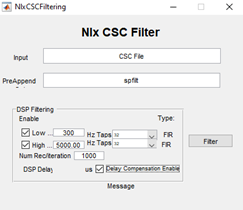
\includegraphics{source_images/sec3.2.1_nix_csc_filter.png}
\caption{Nix csc filter}
\end{figure}

\begin{enumerate}
\def\labelenumi{\arabic{enumi}.}
\setcounter{enumi}{2}
\item
  Examine the filtered traces:

  \begin{enumerate}
  \def\labelenumii{\arabic{enumii}.}
  \tightlist
  \item
    Take a closer look at the filtered traces (Open in \texttt{Neuraview} on any
    Windows machine) and determine which channels are likely to have
    isolatable spikes and how many distinct spikes there might be. It helps
    to keep \texttt{Neuraview} open when setting thresholds in the next step.
  \end{enumerate}
\item
  Spike detection from filtered traces:

  \begin{enumerate}
  \def\labelenumii{\arabic{enumii}.}
  \item
    Use the \texttt{CSCSpikeExtractor} tool on any Windows machine to detect spikes
    above or below a given µV) threshold. The units displayed in the program
    will be AdBitVolts which are simply 10.92x from the µV value.
  \item
    Based on the filtered traces, within \texttt{CSCSpikeExtractor}, set the spike
    extraction properties (\texttt{Spike\ Extraction\ -\textgreater{}\ Properties} OR \texttt{Ctrl+P}) as
    shown above. The \texttt{Extraction\ Value} is set to 10.92x the µV you chose by
    viewing the filtered traces.
  \item
    Press \texttt{Ctrl+S} to extract spikes from the selected file at the desired
    settings. The resulting file will be placed in the \texttt{extracted\ spikes}
    filter on the \texttt{Desktop}.
  \item
    Create subfolders in the recording folder for each threshold and move
    the extracted spikes at each threshold into the appropriate folder.
    These spike-detected files will be used for spike sorting in the next
    step.
  \item
    \textbf{If it helps with detecting real spike waveforms while eliminating
    noise, run recordings through spike detection at multiple threshold
    (positive or negative) such that only all putative neurons are accounted
    for a minimal noise is detected.}
  \end{enumerate}
\end{enumerate}

\begin{figure}
\centering
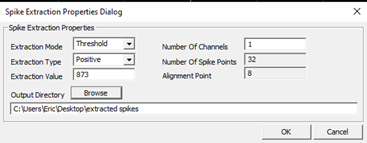
\includegraphics{source_images/sec3.2.2_spike_extraction_properties.png}
\caption{Spike extraction
properties}
\end{figure}

\begin{enumerate}
\def\labelenumi{\arabic{enumi}.}
\setcounter{enumi}{4}
\item
  Spike sorting:

  \begin{enumerate}
  \def\labelenumii{\arabic{enumii}.}
  \item
    Open the extracted spikes in \texttt{Spikesort3D} on either the Neuralynx
    machine or another Windows machine that has an active \texttt{SpikeSort3D}
    licence. You can also use \texttt{TeamViewer} to control the Neuralynx machine
    but this works much better with another Windows machine.
  \item
    Press OK when the feature selection window appears. If you want to
    select alternate features to display, select them from the list
    provided. Sometimes it can be helpful to use PCA1 -- 3 in isolating
    neurons but often it makes things more challenging.
  \item
    Using the 3D Plot, examine the clustering of spikes. Follow the image
    below to aid in interacting with the 3D plot (MB = the scroll wheel
    button i.e.~middle mouse button). You can change the features displayed
    on each axis with \texttt{Q/W}, \texttt{A/S}, and \texttt{Z/X} respectively. Also, \texttt{Ctrl+P}
    brings up a window that allows you to change the size and opacity of
    points on the plot (I find \texttt{size\ =\ 2}, \texttt{alpha\ =\ 0.5} works well to
    improve visual definition of the clusters). If distinct clusters are
    difficult to see, find the combination of 3 features that produces the
    most noticeable clustering or the greatest spread of points in the
    space. The features displayed in the 3D plot are shown at the top left
    of the plot (i.e.~X(3) Height \# \# \# \#). Use those features for the
    next step. 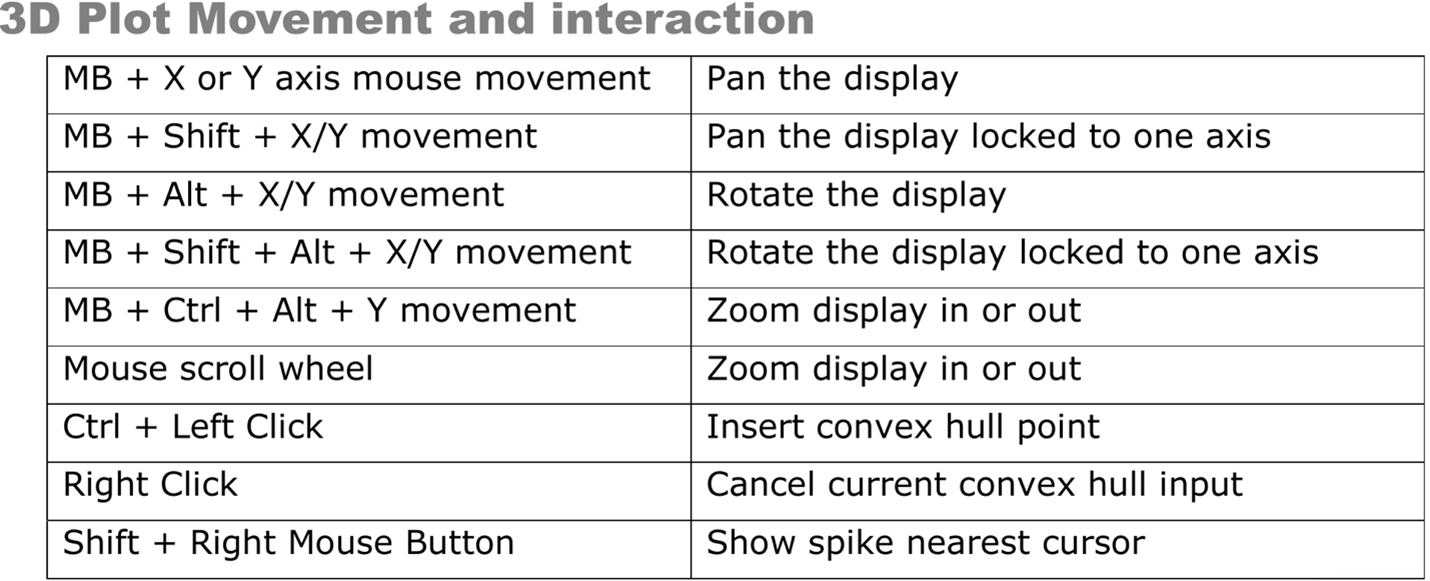
\includegraphics{source_images/sec3.2.3_3d_plot_movement.png}
  \item
    Run \texttt{KlustaKwik} (\texttt{Cluster\ →\ Autocluster\ using\ KlustaKwik}) and select
    the 3 features that generate the most clearly separable clusters on the
    3D view -- often, the first 3 (\texttt{Peak}, \texttt{Valley}, \texttt{Energy}) do a decent
    job. Change the \texttt{MaxPossibleClusters} to \texttt{10} before pressing \texttt{Run}. The
    remaining settings should match the image below. 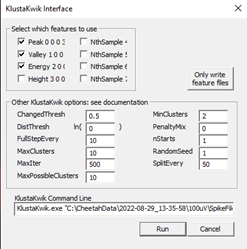
\includegraphics{source_images/sec3.2.4_klustakwik.png}
  \item
    Following calculations, use the \texttt{Waveform} window and the 3D plot to
    group the distinct clusters into what you believe are waveforms produced
    by distinct neurons. Use the number keys to highlight distinct clusters
    and \texttt{Ctrl+M} to merge clusters together. \texttt{Ctrl+C} copies the selected
    cluster and can be used to split a cluster into 2 if you believe
    portions of the cluster belong to distinct putative neurons. This step
    takes some practice. You can use \texttt{Ctrl+Z} to undo only one move.
    Otherwise, you may need to exit without saving and start again at
    step 4. Save with \texttt{Ctrl+S} often and click OK to overwrite the file.
  \item
    Once you are satisfied with the waveforms left, note how many there are,
    and whether it seems possible that some of the groups belong to the same
    neuron. Consider what you know about excitable membranes to make these
    decisions. Fill out the \texttt{Spike\ Sorting\ Database} with the information
    used to reach this point. This includes, the threshold(s), \# of
    clusters, \# of putative neurons (often 1 less than the \# of clusters
    because it would be a stretch to include the smallest amplitude waveform
    as a distinct, separable neuron), and any else to note from performing
    sorting.
  \item
    Save each cluster to its own spike file
    (\texttt{File\ →\ Save\ Multiple\ Spike\ Files})
  \item
    Open the separate spike files you just created, along with the original
    filtered trace in \texttt{Neuraview}. Scroll along the recording and examine if
    the sorting you performed seems believable. Do the spikes in different
    rows really seem like they're different in the filtered trace? Do some
    spikes not seem like real spikes? If anything seems amiss, make the
    appropriate merges in \texttt{SpikeSort3D} before proceding.
  \item
    Export the relevant data from the sorting. Perform the following:

    \begin{enumerate}
    \def\labelenumiii{\arabic{enumiii}.}
    \item
      \texttt{File\ →\ Save\ ASCII\ Timestamp\ Files}
    \item
      \texttt{File\ →\ Save\ Multiple\ Spike\ Files}
    \item
      \texttt{File\ →\ Save\ ASCII\ Avg\ Waveforms}
    \item
      Also, save the file itself with \texttt{Ctrl+S}
    \end{enumerate}
  \item
    Lastly, bring up all the waveforms together on the waveform plot. Take a
    screenshot and save it to the folder where the extracted spikes (and now
    timestamps files) are stored.
  \end{enumerate}
\item
  Moving sorted files to other locations:

  \begin{enumerate}
  \def\labelenumii{\arabic{enumii}.}
  \item
    Once a chunk of recordings have been sorted, copy/paste the entire
    recording file to Eric's orange 1TB storage drive (Lacie). Place them in
    the following folder:

    \texttt{Eric\textquotesingle{}s\ data/sorted\_recordings}
  \end{enumerate}
\end{enumerate}

\hypertarget{raw-data-and-spike-sorted-traces}{%
\chapter{Raw data and spike sorted traces}\label{raw-data-and-spike-sorted-traces}}

This is an R Markdown document. Markdown is a simple formatting syntax for authoring HTML, PDF, and MS Word documents. For more details on using R Markdown see \url{http://rmarkdown.rstudio.com}.

When you click the \textbf{Knit} button a document will be generated that includes both content as well as the output of any embedded R code chunks within the document. You can embed an R code chunk like this:

\begin{Shaded}
\begin{Highlighting}[]
\FunctionTok{summary}\NormalTok{(cars)}
\end{Highlighting}
\end{Shaded}

\begin{verbatim}
##      speed           dist       
##  Min.   : 4.0   Min.   :  2.00  
##  1st Qu.:12.0   1st Qu.: 26.00  
##  Median :15.0   Median : 36.00  
##  Mean   :15.4   Mean   : 42.98  
##  3rd Qu.:19.0   3rd Qu.: 56.00  
##  Max.   :25.0   Max.   :120.00
\end{verbatim}

\hypertarget{including-plots}{%
\section{Including Plots}\label{including-plots}}

You can also embed plots, for example:

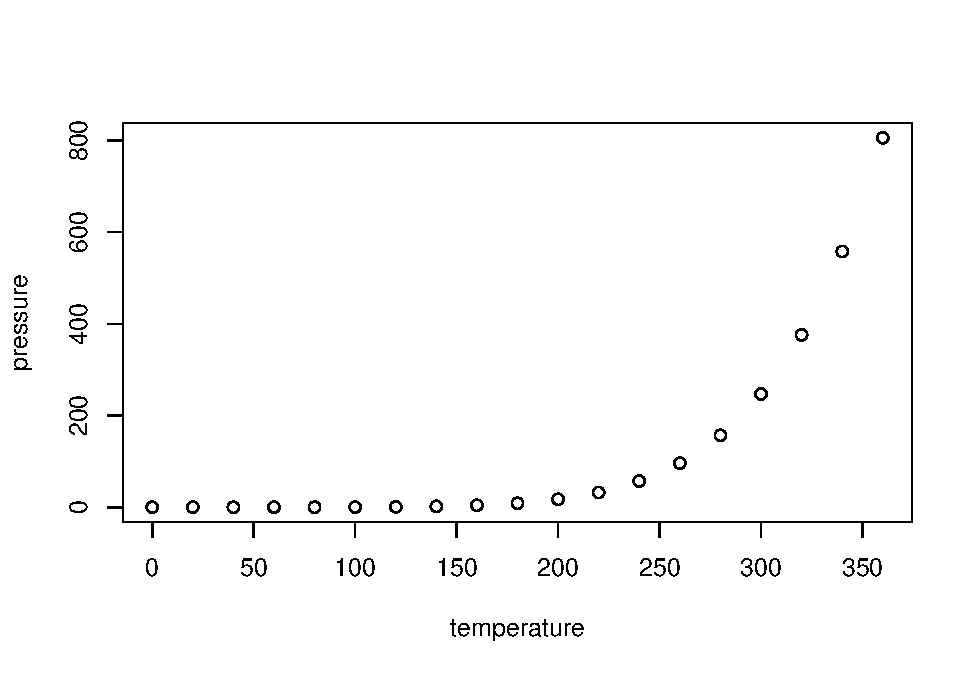
\includegraphics{_main_files/figure-latex/pressure2-1.pdf}

Note that the \texttt{echo\ =\ FALSE} parameter was added to the code chunk to prevent printing of the R code that generated the plot.

\hypertarget{data-wrangling}{%
\chapter{Data wrangling}\label{data-wrangling}}

Once data have been spike sorted, we are ready to begin working in \texttt{R}. To get
to a point where meaningful preliminary plots can be produced, a few things need
to be addressed:

\begin{enumerate}
\def\labelenumi{\arabic{enumi})}
\item
  Labeling the time series of spike \& photodiode data based on the stimulus
  that appears on screen (i.e., matching the log file to the data file). This
  includes labeling phases (like ``blank'', ``stationary'', and ``moving'') along
  with experimental metadata such as SF, TF, and stimulus orientation
  (direction).
\item
  Re-organizing the spike \& photodiode so that separate replicates of a
  stimulus run are uniquely labelled and then arranged together.
\item
  Binning the data into 10- and 100-ms data sets, and then exporting CSVs of
  the unbinned, 10-ms-binned, and 100-ms-binned data. This will be highly
  useful for situations where you are handling multiple data files (e.g., from
  different recording days), in which case it is likely that your machine will
  not be able to store all objects in RAM.
\end{enumerate}

\begin{quote}
Before proceeding any further, please ensure you have installed and loaded all
the necessary \texttt{R} packages as detailed in the Preface section of this guide.
\end{quote}

\hypertarget{import-example-file-and-metadata}{%
\section{Import example file and metadata}\label{import-example-file-and-metadata}}

We will use a recently-collected data file and its corresponding metadata file
to showcase the fundamentals of wrangling ephys data into a more easily
plot-able format.

\hypertarget{identify-files-to-import}{%
\subsection{Identify files to import}\label{identify-files-to-import}}

The following code is based on the assumptions that: 1) Your files are stored in
a directory entitled \texttt{/data} 2) The basename of each file (i.e., the name of the
file, excluding the file extension) is identical for each set of spike sorted
data and corresponding metadata log file (e.g., \texttt{04132022\_009m.mat} and
\texttt{04132022\_009m} have the same basename, which is \texttt{04132022\_009m}).

\begin{Shaded}
\begin{Highlighting}[]
\DocumentationTok{\#\# List all files of each file type}
\NormalTok{csv\_files }\OtherTok{\textless{}{-}}
  \FunctionTok{list.files}\NormalTok{(}\StringTok{"./data"}\NormalTok{, }\AttributeTok{pattern =} \StringTok{".csv"}\NormalTok{,}
             \AttributeTok{full.names =} \ConstantTok{TRUE}\NormalTok{)}
\NormalTok{mat\_files }\OtherTok{\textless{}{-}}
  \FunctionTok{list.files}\NormalTok{(}\StringTok{"./data"}\NormalTok{, }\AttributeTok{pattern =} \StringTok{".mat"}\NormalTok{,}
             \AttributeTok{full.names =} \ConstantTok{TRUE}\NormalTok{)}

\DocumentationTok{\#\# Generate metadata tibbles for each file type}
\NormalTok{csv\_file\_info }\OtherTok{\textless{}{-}}
  \FunctionTok{tibble}\NormalTok{(}
    \AttributeTok{csv\_files =}\NormalTok{ csv\_files,}
    \DocumentationTok{\#\# Extract the basename by removing the file extension}
    \AttributeTok{basename =}  \FunctionTok{basename}\NormalTok{(csv\_files) }\SpecialCharTok{\%\textgreater{}\%} \FunctionTok{str\_remove}\NormalTok{(}\StringTok{".csv"}\NormalTok{),}
    \DocumentationTok{\#\# }\AlertTok{NOTE}\DocumentationTok{: PLEASE ADJUST THE FOLLOWING LINE TO BE ABLE TO EXCTRACT OUT THE}
    \DocumentationTok{\#\# DATE BASED ON YOUR NAMING CONVENTION}
    \AttributeTok{basedate =}  \FunctionTok{basename}\NormalTok{(csv\_files) }\SpecialCharTok{\%\textgreater{}\%} \FunctionTok{str\_sub}\NormalTok{(}\AttributeTok{start =} \DecValTok{1}\NormalTok{, }\AttributeTok{end =} \DecValTok{12}\NormalTok{)}
\NormalTok{  )}
\NormalTok{mat\_file\_info }\OtherTok{\textless{}{-}}
  \FunctionTok{tibble}\NormalTok{(}
    \AttributeTok{mat\_files =}\NormalTok{ mat\_files,}
    \DocumentationTok{\#\# Extract the basename by removing the file extension}
    \AttributeTok{basename =}  \FunctionTok{basename}\NormalTok{(mat\_files) }\SpecialCharTok{\%\textgreater{}\%} \FunctionTok{str\_remove}\NormalTok{(}\StringTok{".mat"}\NormalTok{),}
    \DocumentationTok{\#\# }\AlertTok{NOTE}\DocumentationTok{: AGAIN, PLEASE ADJUST THE FOLLOWING LINE TO BE ABLE TO EXCTRACT OUT}
    \DocumentationTok{\#\# THE DATE BASED ON YOUR NAMING CONVENTION}
    \AttributeTok{basedate =}  \FunctionTok{basename}\NormalTok{(mat\_files) }\SpecialCharTok{\%\textgreater{}\%} \FunctionTok{str\_sub}\NormalTok{(}\AttributeTok{start =} \DecValTok{1}\NormalTok{, }\AttributeTok{end =} \DecValTok{12}\NormalTok{)}
\NormalTok{  )}

\DocumentationTok{\#\# Matchmake between .MAT data and .CSV log files}
\NormalTok{csv\_mat\_filejoin }\OtherTok{\textless{}{-}}
  \FunctionTok{inner\_join}\NormalTok{(csv\_file\_info, mat\_file\_info, }\AttributeTok{by =} \StringTok{"basename"}\NormalTok{) }\SpecialCharTok{\%\textgreater{}\%}
  \DocumentationTok{\#\# OPTIONAL STEP: remove any rows where either the .MAT or .CSV is missing}
  \FunctionTok{drop\_na}\NormalTok{()}

\DocumentationTok{\#\# Store a vector of basenames in the environment. This will become useful later}
\NormalTok{base\_names }\OtherTok{\textless{}{-}}\NormalTok{ csv\_mat\_filejoin}\SpecialCharTok{$}\NormalTok{basename}

\DocumentationTok{\#\# Your end products from this code block should look something like:}
\NormalTok{csv\_mat\_filejoin}
\end{Highlighting}
\end{Shaded}

\begin{verbatim}
## # A tibble: 1 x 5
##   csv_files                basename      basedate.x   mat_files          based~1
##   <chr>                    <chr>         <chr>        <chr>              <chr>  
## 1 ./data/04132022_009m.csv 04132022_009m 04132022_009 ./data/04132022_0~ 041320~
## # ... with abbreviated variable name 1: basedate.y
\end{verbatim}

\begin{Shaded}
\begin{Highlighting}[]
\DocumentationTok{\#\# and:}
\NormalTok{base\_names}
\end{Highlighting}
\end{Shaded}

\begin{verbatim}
## [1] "04132022_009m"
\end{verbatim}

\hypertarget{data-import-and-preliminary-labeling}{%
\subsection{Data import and preliminary labeling}\label{data-import-and-preliminary-labeling}}

We will now use the \texttt{R.matlab} package to import the \texttt{.mat} file into R and then
label the spike and photodiode time series based on the information in the
\texttt{.csv} log file

Because \texttt{.mat} files can be large, data import can take several minutes.

Please see in-line comments for further guidance

\begin{Shaded}
\begin{Highlighting}[]
\DocumentationTok{\#\# Tidy up how R has been using RAM by running garbage collection}
\FunctionTok{gc}\NormalTok{()}
\end{Highlighting}
\end{Shaded}

\begin{verbatim}
##           used  (Mb) gc trigger  (Mb) max used  (Mb)
## Ncells 2437148 130.2    4173244 222.9  4173244 222.9
## Vcells 4211242  32.2   10146329  77.5  8020311  61.2
\end{verbatim}

\begin{Shaded}
\begin{Highlighting}[]
\DocumentationTok{\#\# Set up empty vectors that will collect sets of replicates that we will be}
\DocumentationTok{\#\# splitting up}
\NormalTok{metadata\_sets }\OtherTok{\textless{}{-}} \ConstantTok{NULL}
\NormalTok{meta\_splits }\OtherTok{\textless{}{-}} \ConstantTok{NULL}
\NormalTok{data\_splits }\OtherTok{\textless{}{-}} \ConstantTok{NULL}

\NormalTok{starttime }\OtherTok{\textless{}{-}} \FunctionTok{Sys.time}\NormalTok{() }\DocumentationTok{\#\# Optional, will help you assess run time}
\ControlFlowTok{for}\NormalTok{ (i }\ControlFlowTok{in} \DecValTok{1}\SpecialCharTok{:}\FunctionTok{nrow}\NormalTok{(csv\_mat\_filejoin)) \{}

  \DocumentationTok{\#\# Which file \# are we working on?}
  \FunctionTok{print}\NormalTok{(i)}

  \DocumentationTok{\#\# Set up temporary objects in which to eventually write data}
\NormalTok{  csv\_data\_sets }\OtherTok{\textless{}{-}} \ConstantTok{NULL}
\NormalTok{  mat\_data\_sets }\OtherTok{\textless{}{-}} \ConstantTok{NULL}
\NormalTok{  joined\_data\_sets }\OtherTok{\textless{}{-}} \ConstantTok{NULL}

  \DocumentationTok{\#\# Import the matlab file. This may take some time}
\NormalTok{  mat\_import }\OtherTok{\textless{}{-}}
\NormalTok{    R.matlab}\SpecialCharTok{::}\FunctionTok{readMat}\NormalTok{(csv\_mat\_filejoin[i,}\StringTok{"mat\_files"}\NormalTok{])}

  \DocumentationTok{\#\# Read in the corresponding csv log file}
\NormalTok{  csv\_data\_sets[[i]] }\OtherTok{\textless{}{-}}
    \FunctionTok{read\_csv}\NormalTok{(}\FunctionTok{as.character}\NormalTok{(csv\_mat\_filejoin[i,}\StringTok{"csv\_files"}\NormalTok{]),}
             \AttributeTok{show\_col\_types =} \ConstantTok{FALSE}\NormalTok{) }\SpecialCharTok{\%\textgreater{}\%}
    \DocumentationTok{\#\# Rename columns for convenience}
    \FunctionTok{rename}\NormalTok{(}
      \AttributeTok{Spatial\_Frequency =} \StringTok{\textasciigrave{}}\AttributeTok{Spatial Frequency}\StringTok{\textasciigrave{}}\NormalTok{,}
      \AttributeTok{Temporal\_Frequency =} \StringTok{\textasciigrave{}}\AttributeTok{Temporal Frequency}\StringTok{\textasciigrave{}}
\NormalTok{    )}
  \DocumentationTok{\#\# Set up a \textasciigrave{}SF\_cpd\textasciigrave{} column that tranlates SFs to cycles per degree}
\NormalTok{  csv\_data\_sets[[i]]}\SpecialCharTok{$}\NormalTok{SF\_cpd[csv\_data\_sets[[i]]}\SpecialCharTok{$}\NormalTok{Spatial\_Frequency }\SpecialCharTok{==} \FloatTok{0.000668}\NormalTok{] }\OtherTok{\textless{}{-}}
    \DecValTok{2}\SpecialCharTok{\^{}{-}}\DecValTok{6}
\NormalTok{  csv\_data\_sets[[i]]}\SpecialCharTok{$}\NormalTok{SF\_cpd[csv\_data\_sets[[i]]}\SpecialCharTok{$}\NormalTok{Spatial\_Frequency }\SpecialCharTok{==} \FloatTok{0.001336}\NormalTok{] }\OtherTok{\textless{}{-}}
    \DecValTok{2}\SpecialCharTok{\^{}{-}}\DecValTok{5}
\NormalTok{  csv\_data\_sets[[i]]}\SpecialCharTok{$}\NormalTok{SF\_cpd[csv\_data\_sets[[i]]}\SpecialCharTok{$}\NormalTok{Spatial\_Frequency }\SpecialCharTok{==} \FloatTok{0.00267}\NormalTok{]  }\OtherTok{\textless{}{-}}
    \DecValTok{2}\SpecialCharTok{\^{}{-}}\DecValTok{4}
\NormalTok{  csv\_data\_sets[[i]]}\SpecialCharTok{$}\NormalTok{SF\_cpd[csv\_data\_sets[[i]]}\SpecialCharTok{$}\NormalTok{Spatial\_Frequency }\SpecialCharTok{==} \FloatTok{0.0053}\NormalTok{]   }\OtherTok{\textless{}{-}}
    \DecValTok{2}\SpecialCharTok{\^{}{-}}\DecValTok{3}
\NormalTok{  csv\_data\_sets[[i]]}\SpecialCharTok{$}\NormalTok{SF\_cpd[csv\_data\_sets[[i]]}\SpecialCharTok{$}\NormalTok{Spatial\_Frequency }\SpecialCharTok{==} \FloatTok{0.0106}\NormalTok{]   }\OtherTok{\textless{}{-}}
    \DecValTok{2}\SpecialCharTok{\^{}{-}}\DecValTok{2}
\NormalTok{  csv\_data\_sets[[i]]}\SpecialCharTok{$}\NormalTok{SF\_cpd[csv\_data\_sets[[i]]}\SpecialCharTok{$}\NormalTok{Spatial\_Frequency }\SpecialCharTok{==} \FloatTok{0.0212}\NormalTok{]   }\OtherTok{\textless{}{-}}
    \DecValTok{2}\SpecialCharTok{\^{}{-}}\DecValTok{1}

  \DocumentationTok{\#\# The log file does not have time = 0, so set up a separate tibble to}
  \DocumentationTok{\#\# add this info in later. Some of the metadata will just be filler for now.}
\NormalTok{  initial }\OtherTok{\textless{}{-}} \FunctionTok{tibble}\NormalTok{(}
    \AttributeTok{Trial =} \StringTok{"initialization"}\NormalTok{,}
    \AttributeTok{Spatial\_Frequency =}\NormalTok{ csv\_data\_sets[[i]]}\SpecialCharTok{$}\NormalTok{Spatial\_Frequency[}\DecValTok{1}\NormalTok{],}
    \AttributeTok{SF\_cpd =}\NormalTok{ csv\_data\_sets[[i]]}\SpecialCharTok{$}\NormalTok{SF\_cpd[}\DecValTok{1}\NormalTok{],}
    \AttributeTok{Temporal\_Frequency =}\NormalTok{ csv\_data\_sets[[i]]}\SpecialCharTok{$}\NormalTok{Temporal\_Frequency[}\DecValTok{1}\NormalTok{],}
    \AttributeTok{Direction  =}\NormalTok{ csv\_data\_sets[[i]]}\SpecialCharTok{$}\NormalTok{Direction[}\DecValTok{1}\NormalTok{],}
    \AttributeTok{Time =} \FloatTok{0.000}
\NormalTok{  )}

  \DocumentationTok{\#\# Determine when the onset of motion occurred according to matlab}
  \DocumentationTok{\#\# }\AlertTok{NOTE}\DocumentationTok{: IF THIS INFO IS NOT IN CHANNEL 3, PLEASE CHANGE ACCCORDINGLY}
\NormalTok{  first\_moving\_mat }\OtherTok{\textless{}{-}}
\NormalTok{    mat\_import[[stringr}\SpecialCharTok{::}\FunctionTok{str\_which}\NormalTok{(}\FunctionTok{names}\NormalTok{(mat\_import), }\StringTok{"Ch3"}\NormalTok{)[}\DecValTok{1}\NormalTok{]]][[}\DecValTok{5}\NormalTok{]][,}\DecValTok{1}\NormalTok{][}\DecValTok{1}\NormalTok{]}
  \DocumentationTok{\#\# Find the first "moving" phase in the log file}
\NormalTok{  first\_moving\_csv }\OtherTok{\textless{}{-}}
\NormalTok{    csv\_data\_sets[[i]] }\SpecialCharTok{\%\textgreater{}\%}
    \FunctionTok{filter}\NormalTok{(Trial }\SpecialCharTok{==} \StringTok{"moving"}\NormalTok{) }\SpecialCharTok{\%\textgreater{}\%}
    \FunctionTok{select}\NormalTok{(Time) }\SpecialCharTok{\%\textgreater{}\%}
    \FunctionTok{slice}\NormalTok{(}\DecValTok{1}\NormalTok{) }\SpecialCharTok{\%\textgreater{}\%}
    \FunctionTok{as.numeric}\NormalTok{()}
  \DocumentationTok{\#\# Find the first "blank" phase in the log file}
\NormalTok{  first\_blank }\OtherTok{\textless{}{-}}
\NormalTok{    csv\_data\_sets[[i]] }\SpecialCharTok{\%\textgreater{}\%}
    \FunctionTok{filter}\NormalTok{(Trial }\SpecialCharTok{==} \StringTok{"blank"}\NormalTok{) }\SpecialCharTok{\%\textgreater{}\%}
    \FunctionTok{select}\NormalTok{(Time) }\SpecialCharTok{\%\textgreater{}\%}
    \FunctionTok{slice}\NormalTok{(}\DecValTok{1}\NormalTok{) }\SpecialCharTok{\%\textgreater{}\%}
    \FunctionTok{as.numeric}\NormalTok{()}
  \DocumentationTok{\#\# Compute the difference between these two}
\NormalTok{  first\_mvbl\_diff }\OtherTok{\textless{}{-}}\NormalTok{ first\_moving\_csv }\SpecialCharTok{{-}}\NormalTok{ first\_blank}

  \DocumentationTok{\#\# Check to see if the final row of the metadata is "moving" and truncate}
  \DocumentationTok{\#\# if not}
  \DocumentationTok{\#\# This can effectively be done by truncating after the final "moving" phase}
\NormalTok{  max\_moving\_sweep }\OtherTok{\textless{}{-}}
    \FunctionTok{max}\NormalTok{(}\FunctionTok{which}\NormalTok{(csv\_data\_sets[[i]]}\SpecialCharTok{$}\NormalTok{Trial }\SpecialCharTok{==} \StringTok{"moving"}\NormalTok{))}

\NormalTok{  first\_csv\_tmp }\OtherTok{\textless{}{-}}
    \FunctionTok{bind\_rows}\NormalTok{(initial, csv\_data\_sets[[i]]) }\SpecialCharTok{\%\textgreater{}\%}
    \DocumentationTok{\#\# Add 1 to max moving sweep since we tacked on "initial" in previous step}
    \DocumentationTok{\#\# Then slice to restrict any extraneous partial sweeps}
    \FunctionTok{slice\_head}\NormalTok{(}\AttributeTok{n =}\NormalTok{ (max\_moving\_sweep }\SpecialCharTok{+} \DecValTok{1}\NormalTok{)) }\SpecialCharTok{\%\textgreater{}\%}
    \DocumentationTok{\#\# Add the first event time to "Time" and subtract first\_mvbl\_diff (\textasciitilde{}2 secs)}
    \FunctionTok{mutate}\NormalTok{(}\AttributeTok{Time =}\NormalTok{ Time }\SpecialCharTok{+}\NormalTok{ first\_moving\_mat }\SpecialCharTok{{-}}\NormalTok{ first\_mvbl\_diff }\SpecialCharTok{{-}}\NormalTok{ first\_blank) }\SpecialCharTok{\%\textgreater{}\%}
    \DocumentationTok{\#\# Make character version of Time for joining later}
    \DocumentationTok{\#\# This will be crucial for \_join functions}
    \FunctionTok{mutate}\NormalTok{(}\AttributeTok{Time\_char =} \FunctionTok{as.character}\NormalTok{(}\FunctionTok{round}\NormalTok{(Time,}\DecValTok{3}\NormalTok{)))}

  \DocumentationTok{\#\# Duplicate the initialization for ease of setting T0}
\NormalTok{  inception }\OtherTok{\textless{}{-}}
\NormalTok{    initial }\SpecialCharTok{\%\textgreater{}\%}
    \FunctionTok{mutate}\NormalTok{(}\AttributeTok{Time\_char =} \FunctionTok{as.character}\NormalTok{(}\FunctionTok{round}\NormalTok{(Time,}\DecValTok{3}\NormalTok{)))}
\NormalTok{  inception}\SpecialCharTok{$}\NormalTok{Trial[}\DecValTok{1}\NormalTok{] }\OtherTok{\textless{}{-}} \StringTok{"inception"}

  \DocumentationTok{\#\# Bind the initialization rows}
\NormalTok{  first\_csv }\OtherTok{\textless{}{-}}
    \FunctionTok{bind\_rows}\NormalTok{(inception, first\_csv\_tmp)}
  \DocumentationTok{\#\# Compute stimulus end times}
\NormalTok{  first\_csv}\SpecialCharTok{$}\NormalTok{Stim\_end }\OtherTok{\textless{}{-}} \FunctionTok{c}\NormalTok{(first\_csv}\SpecialCharTok{$}\NormalTok{Time[}\SpecialCharTok{{-}}\DecValTok{1}\NormalTok{], }\FunctionTok{max}\NormalTok{(first\_csv}\SpecialCharTok{$}\NormalTok{Time) }\SpecialCharTok{+} \DecValTok{3}\NormalTok{)}

  \DocumentationTok{\#\# Get final time}
\NormalTok{  final\_time }\OtherTok{\textless{}{-}}\NormalTok{ first\_csv}\SpecialCharTok{$}\NormalTok{Stim\_end[}\FunctionTok{nrow}\NormalTok{(first\_csv)]}

  \DocumentationTok{\#\# Find photodiode}
  \DocumentationTok{\#\# It is almost always in channel 2, but we should be sure to check before}
  \DocumentationTok{\#\# extracting automatically}
\NormalTok{  photod\_default\_channel }\OtherTok{\textless{}{-}}
\NormalTok{    mat\_import[[stringr}\SpecialCharTok{::}\FunctionTok{str\_which}\NormalTok{(}\FunctionTok{names}\NormalTok{(mat\_import), }\StringTok{"Ch2"}\NormalTok{)[}\DecValTok{1}\NormalTok{]]]}
  \ControlFlowTok{if}\NormalTok{ (}\SpecialCharTok{!}\NormalTok{photod\_default\_channel[}\DecValTok{1}\NormalTok{][[}\DecValTok{1}\NormalTok{]][}\DecValTok{1}\NormalTok{] }\SpecialCharTok{==} \StringTok{"waveform"}\NormalTok{) \{}
    \FunctionTok{warning}\NormalTok{(}\StringTok{"File "}\NormalTok{, i,}\StringTok{": Photodiode channel identity uncertain"}\NormalTok{)}
\NormalTok{  \}}

  \DocumentationTok{\#\# Find spikes}
  \DocumentationTok{\#\# Similarly, spikes are almost always in channel 5, but we should check}
\NormalTok{  spikes\_default\_channel }\OtherTok{\textless{}{-}}
\NormalTok{    mat\_import[[stringr}\SpecialCharTok{::}\FunctionTok{str\_which}\NormalTok{(}\FunctionTok{names}\NormalTok{(mat\_import), }\StringTok{"Ch5"}\NormalTok{)[}\DecValTok{1}\NormalTok{]]]}
  \ControlFlowTok{if}\NormalTok{(}\StringTok{"codes"} \SpecialCharTok{\%not\_in\%} \FunctionTok{attributes}\NormalTok{(spikes\_default\_channel)}\SpecialCharTok{$}\NormalTok{dimnames[[}\DecValTok{1}\NormalTok{]]) \{}
    \FunctionTok{warning}\NormalTok{(}\StringTok{"File "}\NormalTok{, i,}\StringTok{": Sorted spikes channel identity uncertain"}\NormalTok{)}
\NormalTok{  \}}
  \DocumentationTok{\#\# If that worked, see if we can automatically determine the "times" and}
  \DocumentationTok{\#\# "codes" slot numbers}
\NormalTok{  times\_location }\OtherTok{\textless{}{-}}
    \FunctionTok{which}\NormalTok{(}\FunctionTok{attributes}\NormalTok{(spikes\_default\_channel)}\SpecialCharTok{$}\NormalTok{dimnames[[}\DecValTok{1}\NormalTok{]] }\SpecialCharTok{==} \StringTok{"times"}\NormalTok{)}
\NormalTok{  codes\_location }\OtherTok{\textless{}{-}}
    \FunctionTok{which}\NormalTok{(}\FunctionTok{attributes}\NormalTok{(spikes\_default\_channel)}\SpecialCharTok{$}\NormalTok{dimnames[[}\DecValTok{1}\NormalTok{]] }\SpecialCharTok{==} \StringTok{"codes"}\NormalTok{)}

  \DocumentationTok{\#\# Extract photodiode data}
  \FunctionTok{options}\NormalTok{(}\AttributeTok{scipen =} \DecValTok{999}\NormalTok{)}
\NormalTok{  photod\_full }\OtherTok{\textless{}{-}}
    \FunctionTok{tibble}\NormalTok{(}
      \AttributeTok{Photod =}
\NormalTok{        photod\_default\_channel[}\DecValTok{9}\NormalTok{][[}\DecValTok{1}\NormalTok{]][, }\DecValTok{1}\NormalTok{])}
\NormalTok{  photod\_full}\SpecialCharTok{$}\NormalTok{Time }\OtherTok{\textless{}{-}}
    \FunctionTok{seq}\NormalTok{(}
      \AttributeTok{from =} \DecValTok{0}\NormalTok{,}
      \AttributeTok{by =} \DecValTok{1} \SpecialCharTok{/} \DecValTok{25000}\NormalTok{,}
      \AttributeTok{length.out =} \FunctionTok{nrow}\NormalTok{(photod\_full)}
\NormalTok{    )}
\NormalTok{  photod\_full }\OtherTok{\textless{}{-}}
\NormalTok{    photod\_full }\SpecialCharTok{\%\textgreater{}\%}
    \FunctionTok{mutate}\NormalTok{(}\AttributeTok{Time\_char =} \FunctionTok{as.character}\NormalTok{(}\FunctionTok{round}\NormalTok{(Time, }\DecValTok{5}\NormalTok{)))}

  \DocumentationTok{\#\# Extract all spike data}
\NormalTok{  all\_spike\_dat }\OtherTok{\textless{}{-}}
    \FunctionTok{tibble}\NormalTok{(}
      \AttributeTok{Time =}
\NormalTok{        spikes\_default\_channel[times\_location][[}\DecValTok{1}\NormalTok{]][, }\DecValTok{1}\NormalTok{],}
      \AttributeTok{code =}
\NormalTok{        spikes\_default\_channel[codes\_location][[}\DecValTok{1}\NormalTok{]][, }\DecValTok{1}\NormalTok{]) }\SpecialCharTok{\%\textgreater{}\%}
    \DocumentationTok{\#\# Get rid of empty rows}
    \FunctionTok{filter}\NormalTok{(code }\SpecialCharTok{\textgreater{}} \DecValTok{0}\NormalTok{) }\SpecialCharTok{\%\textgreater{}\%}
    \DocumentationTok{\#\# Characterize time, for purposes of joining later}
    \FunctionTok{mutate}\NormalTok{(}\AttributeTok{Time\_char =} \FunctionTok{as.character}\NormalTok{(}\FunctionTok{round}\NormalTok{(Time, }\DecValTok{5}\NormalTok{))) }\CommentTok{\#\%\textgreater{}\%}
    \CommentTok{\#mutate(code = as.character(code))}

  \DocumentationTok{\#\# How many distinct neurons are there?}
\NormalTok{  n\_cells }\OtherTok{\textless{}{-}} \FunctionTok{sort}\NormalTok{(}\FunctionTok{unique}\NormalTok{(all\_spike\_dat}\SpecialCharTok{$}\NormalTok{code))}

  \ControlFlowTok{if}\NormalTok{(}\FunctionTok{length}\NormalTok{(n\_cells) }\SpecialCharTok{\textgreater{}} \DecValTok{1}\NormalTok{) \{}
\NormalTok{    all\_spike\_dat\_tmp }\OtherTok{\textless{}{-}}
\NormalTok{      all\_spike\_dat }\SpecialCharTok{\%\textgreater{}\%}
      \DocumentationTok{\#\# Group by identity of spiking neuron}
      \FunctionTok{group\_by}\NormalTok{(code) }\SpecialCharTok{\%\textgreater{}\%}
      \DocumentationTok{\#\# Split into separate dfs, one per neuron}
      \CommentTok{\#split(factor(all\_spike\_dat$code))}
      \FunctionTok{group\_split}\NormalTok{()}

    \DocumentationTok{\#\# Keep the name of the first cell\textquotesingle{}s spike column as simply "Spikes"}
\NormalTok{    first\_cell }\OtherTok{\textless{}{-}}
\NormalTok{      all\_spike\_dat\_tmp[[}\DecValTok{1}\NormalTok{]] }\SpecialCharTok{\%\textgreater{}\%}
      \FunctionTok{rename}\NormalTok{(}\AttributeTok{Spikes =}\NormalTok{ code)}

    \DocumentationTok{\#\# Additional cells are labeled as "Spike\_n"}
\NormalTok{    ad\_cells }\OtherTok{\textless{}{-}}\NormalTok{ n\_cells[n\_cells }\SpecialCharTok{\textgreater{}} \DecValTok{1}\NormalTok{]}
\NormalTok{    all\_cells }\OtherTok{\textless{}{-}} \ConstantTok{NULL}
    \ControlFlowTok{for}\NormalTok{ (j }\ControlFlowTok{in}\NormalTok{ ad\_cells) \{}
      \CommentTok{\#print(i)}
\NormalTok{      new\_name }\OtherTok{=} \FunctionTok{paste0}\NormalTok{(}\StringTok{"Spikes\_"}\NormalTok{, j)}
\NormalTok{      all\_cells[[j]] }\OtherTok{\textless{}{-}}
\NormalTok{        all\_spike\_dat\_tmp[[j]]}
      \FunctionTok{names}\NormalTok{(all\_cells[[j]])[}\FunctionTok{match}\NormalTok{(}\StringTok{"code"}\NormalTok{, }\FunctionTok{names}\NormalTok{(all\_cells[[j]]))] }\OtherTok{\textless{}{-}}
\NormalTok{        new\_name}
\NormalTok{    \}}

    \DocumentationTok{\#\# Add first cell back in}
\NormalTok{    all\_cells[[}\DecValTok{1}\NormalTok{]] }\OtherTok{\textless{}{-}}\NormalTok{ first\_cell}

    \DocumentationTok{\#\# Consolidate}
\NormalTok{    all\_spike\_dat }\OtherTok{\textless{}{-}}
\NormalTok{      all\_cells }\SpecialCharTok{\%\textgreater{}\%}
      \DocumentationTok{\#\# Tack on additional spike columns}
      \FunctionTok{reduce}\NormalTok{(left\_join, }\AttributeTok{by =} \StringTok{"Time\_char"}\NormalTok{) }\SpecialCharTok{\%\textgreater{}\%}
      \DocumentationTok{\#\# Remove time.n columns but}
      \DocumentationTok{\#\# Do not remove Time\_char}
      \FunctionTok{select}\NormalTok{(}\SpecialCharTok{{-}}\FunctionTok{contains}\NormalTok{(}\StringTok{"Time."}\NormalTok{)) }\SpecialCharTok{\%\textgreater{}\%}
      \DocumentationTok{\#\# Regenerate numeric time}
      \FunctionTok{mutate}\NormalTok{(}
        \AttributeTok{Time =} \FunctionTok{as.numeric}\NormalTok{(Time\_char)}
\NormalTok{      ) }\SpecialCharTok{\%\textgreater{}\%}
      \FunctionTok{select}\NormalTok{(Time, Time\_char, }\FunctionTok{everything}\NormalTok{())}

\NormalTok{  \} }\ControlFlowTok{else}\NormalTok{ \{}
\NormalTok{    all\_spike\_dat }\OtherTok{\textless{}{-}}
\NormalTok{      all\_spike\_dat }\SpecialCharTok{\%\textgreater{}\%}
      \FunctionTok{rename}\NormalTok{(}\AttributeTok{Spikes =}\NormalTok{ code) }\SpecialCharTok{\%\textgreater{}\%}
      \FunctionTok{select}\NormalTok{(Time, Time\_char, }\FunctionTok{everything}\NormalTok{())}
\NormalTok{  \}}

  \FunctionTok{options}\NormalTok{(}\AttributeTok{scipen =} \DecValTok{999}\NormalTok{)}
\NormalTok{  mat\_data\_sets[[i]] }\OtherTok{\textless{}{-}}
    \DocumentationTok{\#\# Generate a time sequence from 0 to final\_time}
    \FunctionTok{tibble}\NormalTok{(}
      \AttributeTok{Time =} \FunctionTok{seq}\NormalTok{(}\AttributeTok{from =} \DecValTok{0}\NormalTok{, }\AttributeTok{to =}\NormalTok{ final\_time, }\AttributeTok{by =} \FloatTok{0.001}\NormalTok{)}
\NormalTok{    ) }\SpecialCharTok{\%\textgreater{}\%}
    \DocumentationTok{\#\# Character{-}ize it}
    \FunctionTok{mutate}\NormalTok{(}\AttributeTok{Time\_char =} \FunctionTok{as.character}\NormalTok{(}\FunctionTok{round}\NormalTok{(Time, }\DecValTok{5}\NormalTok{))) }\SpecialCharTok{\%\textgreater{}\%}
    \DocumentationTok{\#\# Join in the photodiode data}
    \FunctionTok{left\_join}\NormalTok{(photod\_full, }\AttributeTok{by =} \StringTok{"Time\_char"}\NormalTok{) }\SpecialCharTok{\%\textgreater{}\%}
    \FunctionTok{select}\NormalTok{(}\SpecialCharTok{{-}}\NormalTok{Time.y) }\SpecialCharTok{\%\textgreater{}\%}
    \FunctionTok{rename}\NormalTok{(}\AttributeTok{Time =}\NormalTok{ Time.x) }\SpecialCharTok{\%\textgreater{}\%}
    \DocumentationTok{\#\# Join in the spike data}
    \FunctionTok{left\_join}\NormalTok{(all\_spike\_dat, }\AttributeTok{by =} \StringTok{"Time\_char"}\NormalTok{) }\SpecialCharTok{\%\textgreater{}\%}
    \FunctionTok{select}\NormalTok{(}\SpecialCharTok{{-}}\NormalTok{Time.y) }\SpecialCharTok{\%\textgreater{}\%}
    \FunctionTok{rename}\NormalTok{(}\AttributeTok{Time =}\NormalTok{ Time.x) }\SpecialCharTok{\%\textgreater{}\%}
    \FunctionTok{filter}\NormalTok{(Time }\SpecialCharTok{\textless{}=}\NormalTok{ final\_time) }\SpecialCharTok{\%\textgreater{}\%}
    \DocumentationTok{\#\# Replace NAs with 0 in the Spike columns only}
    \FunctionTok{mutate}\NormalTok{(}
      \FunctionTok{across}\NormalTok{(}\FunctionTok{starts\_with}\NormalTok{(}\StringTok{"Spikes"}\NormalTok{), }\SpecialCharTok{\textasciitilde{}}\FunctionTok{replace\_na}\NormalTok{(.x, }\DecValTok{0}\NormalTok{))}
\NormalTok{    )}

  \DocumentationTok{\#\# Merge the matlab data with the metadata}
\NormalTok{  joined\_one\_full }\OtherTok{\textless{}{-}}
\NormalTok{    mat\_data\_sets[[i]] }\SpecialCharTok{\%\textgreater{}\%}
    \DocumentationTok{\#\# Join by the character version of time NOT the numerical!!}
    \FunctionTok{full\_join}\NormalTok{(first\_csv, }\AttributeTok{by =} \StringTok{"Time\_char"}\NormalTok{) }\SpecialCharTok{\%\textgreater{}\%}
    \DocumentationTok{\#\# Rename columns for clarity of reference}
    \FunctionTok{rename}\NormalTok{(}\AttributeTok{Time\_mat =}\NormalTok{ Time.x,}
           \AttributeTok{Time\_csv =}\NormalTok{ Time.y) }\SpecialCharTok{\%\textgreater{}\%}
    \DocumentationTok{\#\# Convert character time to numeric time}
    \FunctionTok{mutate}\NormalTok{(}\AttributeTok{Time =} \FunctionTok{as.numeric}\NormalTok{(Time\_char)) }\SpecialCharTok{\%\textgreater{}\%}
    \DocumentationTok{\#\# Carry metadata forward}
    \FunctionTok{mutate}\NormalTok{(}
      \AttributeTok{Trial =}\NormalTok{ zoo}\SpecialCharTok{::}\FunctionTok{na.locf}\NormalTok{(Trial, }\AttributeTok{type =} \StringTok{"locf"}\NormalTok{),}
      \AttributeTok{Spatial\_Frequency =}\NormalTok{ zoo}\SpecialCharTok{::}\FunctionTok{na.locf}\NormalTok{(Spatial\_Frequency, }\AttributeTok{type =} \StringTok{"locf"}\NormalTok{),}
      \AttributeTok{SF\_cpd =}\NormalTok{ zoo}\SpecialCharTok{::}\FunctionTok{na.locf}\NormalTok{(SF\_cpd, }\AttributeTok{type =} \StringTok{"locf"}\NormalTok{),}
      \AttributeTok{Temporal\_Frequency =}\NormalTok{ zoo}\SpecialCharTok{::}\FunctionTok{na.locf}\NormalTok{(Temporal\_Frequency, }\AttributeTok{type =} \StringTok{"locf"}\NormalTok{),}
      \AttributeTok{Direction =}\NormalTok{ zoo}\SpecialCharTok{::}\FunctionTok{na.locf}\NormalTok{(Direction, }\AttributeTok{type =} \StringTok{"locf"}\NormalTok{),}
      \AttributeTok{Time\_csv =}\NormalTok{ zoo}\SpecialCharTok{::}\FunctionTok{na.locf}\NormalTok{(Time\_csv, }\AttributeTok{type =} \StringTok{"locf"}\NormalTok{),}
      \AttributeTok{Stim\_end =}\NormalTok{ zoo}\SpecialCharTok{::}\FunctionTok{na.locf}\NormalTok{(Stim\_end, }\AttributeTok{type =} \StringTok{"locf"}\NormalTok{)}
\NormalTok{    ) }\SpecialCharTok{\%\textgreater{}\%}
    \DocumentationTok{\#\# Calculate velocity}
    \FunctionTok{mutate}\NormalTok{(}
      \AttributeTok{Speed =}\NormalTok{ Temporal\_Frequency}\SpecialCharTok{/}\NormalTok{SF\_cpd,}
      \AttributeTok{Log2\_Speed =} \FunctionTok{log2}\NormalTok{(Speed)}
\NormalTok{    )}

  \DocumentationTok{\#\# Add info to metadata}
\NormalTok{  metadata\_one\_full }\OtherTok{\textless{}{-}}
\NormalTok{    first\_csv }\SpecialCharTok{\%\textgreater{}\%}
    \FunctionTok{mutate}\NormalTok{(}
      \AttributeTok{Speed =}\NormalTok{ Temporal\_Frequency}\SpecialCharTok{/}\NormalTok{SF\_cpd,}
      \AttributeTok{Log2\_Speed =} \FunctionTok{log2}\NormalTok{(Speed),}
      \AttributeTok{Stim\_end\_diff =} \FunctionTok{c}\NormalTok{(}\DecValTok{0}\NormalTok{, }\FunctionTok{diff}\NormalTok{(Stim\_end))}
\NormalTok{    )}

  \DocumentationTok{\#\# Some quality control checks}
  \DocumentationTok{\#\# What are the stim time differences?}
\NormalTok{  stimtime\_diffs }\OtherTok{\textless{}{-}} \FunctionTok{round}\NormalTok{(metadata\_one\_full}\SpecialCharTok{$}\NormalTok{Stim\_end\_diff)[}\SpecialCharTok{{-}}\FunctionTok{c}\NormalTok{(}\DecValTok{1}\SpecialCharTok{:}\DecValTok{2}\NormalTok{)]}
  \DocumentationTok{\#\# How many total reps were recorded?}
\NormalTok{  stimtime\_reps }\OtherTok{\textless{}{-}} \FunctionTok{length}\NormalTok{(stimtime\_diffs)}\SpecialCharTok{/}\DecValTok{3}
  \DocumentationTok{\#\# What do we expect the overall structure to look like?}
\NormalTok{  stimtime\_expectation }\OtherTok{\textless{}{-}} \FunctionTok{rep}\NormalTok{(}\FunctionTok{c}\NormalTok{(}\DecValTok{1}\NormalTok{,}\DecValTok{1}\NormalTok{,}\DecValTok{3}\NormalTok{), stimtime\_reps)}
  \DocumentationTok{\#\# Does reality match our expectations?}
  \ControlFlowTok{if}\NormalTok{ (}\SpecialCharTok{!}\FunctionTok{all}\NormalTok{(stimtime\_diffs }\SpecialCharTok{==}\NormalTok{ stimtime\_expectation)) \{}
    \DocumentationTok{\#\# If you get this, investigate the file further and determine what went}
    \DocumentationTok{\#\# wrong}
    \FunctionTok{print}\NormalTok{(}\StringTok{"stimtime issue; investigate"}\NormalTok{)}
\NormalTok{  \}}

  \DocumentationTok{\#\# Sometimes the final sweep gets carried for an indefinite amount of time}
  \DocumentationTok{\#\# before the investigator manually shuts things off. The following block}
  \DocumentationTok{\#\# truncates accordingly}
\NormalTok{  mark\_for\_removal }\OtherTok{\textless{}{-}}
    \FunctionTok{which}\NormalTok{(}\FunctionTok{round}\NormalTok{(metadata\_one\_full}\SpecialCharTok{$}\NormalTok{Stim\_end\_diff) }\SpecialCharTok{\%not\_in\%} \FunctionTok{c}\NormalTok{(}\DecValTok{1}\NormalTok{, }\DecValTok{3}\NormalTok{))}
  \ControlFlowTok{if}\NormalTok{ (}\FunctionTok{any}\NormalTok{(mark\_for\_removal }\SpecialCharTok{==} \DecValTok{1} \SpecialCharTok{|}\NormalTok{ mark\_for\_removal }\SpecialCharTok{==} \DecValTok{2}\NormalTok{)) \{}
\NormalTok{    mark\_for\_removal }\OtherTok{\textless{}{-}}\NormalTok{ mark\_for\_removal[mark\_for\_removal }\SpecialCharTok{\textgreater{}} \DecValTok{2}\NormalTok{]}
\NormalTok{  \}}
  \ControlFlowTok{if}\NormalTok{ (}\FunctionTok{length}\NormalTok{(mark\_for\_removal) }\SpecialCharTok{\textgreater{}} \DecValTok{0}\NormalTok{) \{}
\NormalTok{    metadata\_sets[[i]] }\OtherTok{\textless{}{-}}
\NormalTok{      metadata\_one\_full }\SpecialCharTok{\%\textgreater{}\%}
      \FunctionTok{filter}\NormalTok{(Time }\SpecialCharTok{\textless{}}\NormalTok{ metadata\_one\_full[mark\_for\_removal[}\DecValTok{1}\NormalTok{],]}\SpecialCharTok{$}\NormalTok{Time)}
\NormalTok{    joined\_data\_sets[[i]] }\OtherTok{\textless{}{-}}
\NormalTok{      joined\_one\_full }\SpecialCharTok{\%\textgreater{}\%}
      \FunctionTok{filter}\NormalTok{(Time\_mat }\SpecialCharTok{\textless{}}\NormalTok{ metadata\_one\_full[mark\_for\_removal[}\DecValTok{1}\NormalTok{],]}\SpecialCharTok{$}\NormalTok{Time)}
\NormalTok{  \} }\ControlFlowTok{else}\NormalTok{ \{}
\NormalTok{    metadata\_sets[[i]] }\OtherTok{\textless{}{-}}
\NormalTok{      metadata\_one\_full}
\NormalTok{    joined\_data\_sets[[i]] }\OtherTok{\textless{}{-}}
\NormalTok{      joined\_one\_full}
\NormalTok{  \}}

  \DocumentationTok{\#\# Organize the metadata for export in the R environment}
\NormalTok{  meta\_splits[[i]] }\OtherTok{\textless{}{-}}
\NormalTok{    metadata\_sets[[i]] }\SpecialCharTok{\%\textgreater{}\%}
    \DocumentationTok{\#\# Get rid of the non{-}sweep info}
    \FunctionTok{filter}\NormalTok{(}\SpecialCharTok{!}\NormalTok{Trial }\SpecialCharTok{==} \StringTok{"inception"}\NormalTok{) }\SpecialCharTok{\%\textgreater{}\%}
    \FunctionTok{filter}\NormalTok{(}\SpecialCharTok{!}\NormalTok{Trial }\SpecialCharTok{==} \StringTok{"initialization"}\NormalTok{) }\SpecialCharTok{\%\textgreater{}\%}
    \DocumentationTok{\#\# Group by trial}
    \CommentTok{\#group\_by(Spatial\_Frequency, Temporal\_Frequency, Direction) \%\textgreater{}\%}
    \DocumentationTok{\#\# Split by trial group}
    \FunctionTok{group\_split}\NormalTok{(Spatial\_Frequency, Temporal\_Frequency, Direction)}

\NormalTok{  data\_splits[[i]] }\OtherTok{\textless{}{-}}
\NormalTok{    joined\_data\_sets[[i]] }\SpecialCharTok{\%\textgreater{}\%}
    \DocumentationTok{\#\# Get rid of the non{-}sweep info}
    \FunctionTok{filter}\NormalTok{(}\SpecialCharTok{!}\NormalTok{Trial }\SpecialCharTok{==} \StringTok{"inception"}\NormalTok{) }\SpecialCharTok{\%\textgreater{}\%}
    \FunctionTok{filter}\NormalTok{(}\SpecialCharTok{!}\NormalTok{Trial }\SpecialCharTok{==} \StringTok{"initialization"}\NormalTok{) }\SpecialCharTok{\%\textgreater{}\%}
    \DocumentationTok{\#\# Group by trial}
    \FunctionTok{group\_by}\NormalTok{(Spatial\_Frequency, Temporal\_Frequency, Direction) }\SpecialCharTok{\%\textgreater{}\%}
    \DocumentationTok{\#\# Split by trial group}
    \FunctionTok{group\_split}\NormalTok{()}

  \DocumentationTok{\#\# Do some cleanup so large objects don\textquotesingle{}t linger in memory}
  \FunctionTok{rm}\NormalTok{(}
\NormalTok{    first\_csv, inception, initial, mat\_import, first\_csv\_tmp,}
\NormalTok{    photod\_default\_channel, spikes\_default\_channel, photod\_full,}
\NormalTok{    all\_spike\_dat, all\_spike\_dat\_tmp, first\_cell, all\_cells,}
\NormalTok{    metadata\_one\_full, joined\_one\_full, joined\_data\_sets,}
\NormalTok{    csv\_data\_sets, mat\_data\_sets}
\NormalTok{  )}
  \FunctionTok{message}\NormalTok{(}\StringTok{"File "}\NormalTok{, i, }\StringTok{": "}\NormalTok{, csv\_mat\_filejoin[i,}\StringTok{"basename"}\NormalTok{], }\StringTok{" imported"}\NormalTok{)}
  \FunctionTok{gc}\NormalTok{()}
\NormalTok{\}}
\end{Highlighting}
\end{Shaded}

\begin{verbatim}
## [1] 1
\end{verbatim}

\begin{Shaded}
\begin{Highlighting}[]
\NormalTok{endtime }\OtherTok{\textless{}{-}} \FunctionTok{Sys.time}\NormalTok{()}
\NormalTok{endtime }\SpecialCharTok{{-}}\NormalTok{ starttime }\DocumentationTok{\#\# Total elapsed time}
\end{Highlighting}
\end{Shaded}

\begin{verbatim}
## Time difference of 2.194635 mins
\end{verbatim}

\begin{Shaded}
\begin{Highlighting}[]
\DocumentationTok{\#\# Tidy up}
\FunctionTok{gc}\NormalTok{()}
\end{Highlighting}
\end{Shaded}

\begin{verbatim}
##            used  (Mb) gc trigger   (Mb)  max used   (Mb)
## Ncells  4074544 217.7   70130373 3745.4  40623809 2169.6
## Vcells 44126215 336.7  460296310 3511.8 719130736 5486.6
\end{verbatim}

\begin{Shaded}
\begin{Highlighting}[]
\DocumentationTok{\#\# Name each data set according to the basename of the file}
\FunctionTok{names}\NormalTok{(metadata\_sets) }\OtherTok{\textless{}{-}}\NormalTok{ csv\_mat\_filejoin}\SpecialCharTok{$}\NormalTok{basename }\CommentTok{\#base\_names}
\FunctionTok{names}\NormalTok{(meta\_splits)   }\OtherTok{\textless{}{-}}\NormalTok{ csv\_mat\_filejoin}\SpecialCharTok{$}\NormalTok{basename }\CommentTok{\#base\_names}
\FunctionTok{names}\NormalTok{(data\_splits)   }\OtherTok{\textless{}{-}}\NormalTok{ csv\_mat\_filejoin}\SpecialCharTok{$}\NormalTok{basename }\CommentTok{\#base\_names}

\DocumentationTok{\#\# Get organized lists of stimuli that were used}
\DocumentationTok{\#\# This will ultimately be used for arranging data by stimuli in a sensible}
\DocumentationTok{\#\# order}
\NormalTok{metadata\_combos }\OtherTok{\textless{}{-}} \ConstantTok{NULL}
\ControlFlowTok{for}\NormalTok{ (i }\ControlFlowTok{in} \DecValTok{1}\SpecialCharTok{:}\FunctionTok{length}\NormalTok{(metadata\_sets)) \{}
\NormalTok{  metadata\_combos[[i]] }\OtherTok{\textless{}{-}}
\NormalTok{    metadata\_sets[[i]] }\SpecialCharTok{\%\textgreater{}\%}
    \DocumentationTok{\#\# Get unique stimulus parameters}
    \FunctionTok{distinct}\NormalTok{(SF\_cpd, Temporal\_Frequency, Speed, Direction) }\SpecialCharTok{\%\textgreater{}\%}
    \FunctionTok{arrange}\NormalTok{(Direction) }\SpecialCharTok{\%\textgreater{}\%}
    \DocumentationTok{\#\# Sort by SF\_cpd (smallest to largest)}
    \FunctionTok{arrange}\NormalTok{(}\FunctionTok{desc}\NormalTok{(SF\_cpd)) }\SpecialCharTok{\%\textgreater{}\%}
    \FunctionTok{mutate}\NormalTok{(}
      \DocumentationTok{\#\# Set a "plot\_order" which provides a running order of stimuli}
      \AttributeTok{plot\_order =} \DecValTok{1}\SpecialCharTok{:}\FunctionTok{length}\NormalTok{(meta\_splits[[i]]),}
      \AttributeTok{name =} \FunctionTok{paste}\NormalTok{(Direction, }\StringTok{"Deg,"}\NormalTok{,  Speed, }\StringTok{"Deg/s"}\NormalTok{)}
\NormalTok{    )}
\NormalTok{\}}
\FunctionTok{names}\NormalTok{(metadata\_combos) }\OtherTok{\textless{}{-}}\NormalTok{ csv\_mat\_filejoin}\SpecialCharTok{$}\NormalTok{basename }\CommentTok{\#base\_names}
\end{Highlighting}
\end{Shaded}

\textbf{What we now have is the following:}

\begin{itemize}
\tightlist
\item
  \texttt{metadata\_sets}: contains a \texttt{list} of \texttt{tibble}s (one per imported file),
  each of which comprises the stimulus log
\item
  \texttt{metadata\_combos}: contains a \texttt{list} of \texttt{tibble}s (one per imported file),
  each of which comprises the stimulus log re-written in a preferred plotting
  order
\item
  \texttt{meta\_splits}: a \texttt{list} of \texttt{list}s. The first level of the \texttt{list}
  corresponds to the file identities. Within each file's \texttt{list}, there is an
  additional set of \texttt{list}s, each of which contains a \texttt{tibble} with the log
  info for a specific stimulus combination. Essentially the same as
  \texttt{metadata\_sets} but split up on a per-stimulus basis.
\item
  \texttt{data\_splits}: another \texttt{list} of \texttt{list}s, arranged in the same hierarchical
  order as \texttt{meta\_splits}. Each tibble herein contains the spike and photodiode
  data from the \texttt{matlab} file on a per-stimulus basis.
\end{itemize}

Note that since we are only using one example file, each of these lists should
only be 1 element long (with the latter two having additional elements within
the first element)

\hypertarget{organizing-replicates-required-and-binning-optional}{%
\section{Organizing replicates (required) and binning (optional)}\label{organizing-replicates-required-and-binning-optional}}

It is common to record several different sweeps of a stimulus to collect
(somewhat) independent replicates of neural responses. The primary task of this
section will be to use the lists from the previous section to gather \& label
replicates of the same stimulus.

A secondary task is to deal with binning, if desired (highly recommended).
Depending on the goals of plotting and/or analyses, it may be wise to work with
either unbinned spike data or to bin the data at a convenient and sensible
interval. I generally choose to work at the following levels:

\begin{enumerate}
\def\labelenumi{\arabic{enumi}.}
\tightlist
\item
  Unbinned
\item
  Bin size = 10 ms
\item
  Bin size = 100 ms
\end{enumerate}

\textbf{Important note:} Rather than provide separate code for each of these 3
scenarios, I will provide one example. Bin size \textbf{must} be declared beforehand
-- please pay attention.

\begin{Shaded}
\begin{Highlighting}[]
\DocumentationTok{\#\# Set bin size here}
\DocumentationTok{\#\# Units are in ms (e.g. 10 = 10ms)}
\NormalTok{bin\_size }\OtherTok{=} \DecValTok{10} \DocumentationTok{\#\# 10 or 100 or 1 (1 = "unbinned")}

\NormalTok{slice\_size }\OtherTok{=} \ConstantTok{NULL}
\NormalTok{slicemin }\OtherTok{=} \ConstantTok{NULL}
\NormalTok{slicemax }\OtherTok{=} \ConstantTok{NULL}
\ControlFlowTok{if}\NormalTok{ (bin\_size }\SpecialCharTok{==} \DecValTok{10}\NormalTok{)\{}
\NormalTok{  slice\_size }\OtherTok{\textless{}{-}} \DecValTok{501}
\NormalTok{  slicemin }\OtherTok{\textless{}{-}} \DecValTok{202}
\NormalTok{  slicemax }\OtherTok{\textless{}{-}} \DecValTok{498}
\NormalTok{\} }\ControlFlowTok{else} \ControlFlowTok{if}\NormalTok{ (bin\_size }\SpecialCharTok{==} \DecValTok{100}\NormalTok{)\{}
\NormalTok{  slice\_size }\OtherTok{\textless{}{-}} \DecValTok{51}
\NormalTok{  slicemin }\OtherTok{\textless{}{-}} \DecValTok{21}
\NormalTok{  slicemax }\OtherTok{\textless{}{-}} \DecValTok{49}
\NormalTok{\} }\ControlFlowTok{else} \ControlFlowTok{if}\NormalTok{ (bin\_size }\SpecialCharTok{==} \DecValTok{1}\NormalTok{)\{}
\NormalTok{  slice\_size }\OtherTok{\textless{}{-}} \ConstantTok{NULL}
\NormalTok{  slicemin }\OtherTok{\textless{}{-}} \ConstantTok{NULL}
\NormalTok{  slicemax }\OtherTok{\textless{}{-}} \ConstantTok{NULL}
\NormalTok{\} }\ControlFlowTok{else}\NormalTok{ \{}
  \FunctionTok{stop}\NormalTok{(}\StringTok{"bin\_size is non{-}standard"}\NormalTok{)}
\NormalTok{\}}


\NormalTok{all\_replicate\_data\_reorganized }\OtherTok{\textless{}{-}}
  \FunctionTok{vector}\NormalTok{(}\AttributeTok{mode =} \StringTok{"list"}\NormalTok{, }\AttributeTok{length =} \FunctionTok{length}\NormalTok{(meta\_splits))}
\NormalTok{name\_sets }\OtherTok{\textless{}{-}}
  \FunctionTok{vector}\NormalTok{(}\AttributeTok{mode =} \StringTok{"list"}\NormalTok{, }\AttributeTok{length =} \FunctionTok{length}\NormalTok{(meta\_splits))}
\FunctionTok{gc}\NormalTok{()}
\end{Highlighting}
\end{Shaded}

\begin{verbatim}
##            used  (Mb) gc trigger   (Mb)  max used   (Mb)
## Ncells  4077439 217.8   56104299 2996.3  40623809 2169.6
## Vcells 44125380 336.7  368237048 2809.5 719130736 5486.6
\end{verbatim}

\begin{Shaded}
\begin{Highlighting}[]
\NormalTok{starttime }\OtherTok{\textless{}{-}} \FunctionTok{Sys.time}\NormalTok{()}
\ControlFlowTok{for}\NormalTok{ (i }\ControlFlowTok{in} \DecValTok{1}\SpecialCharTok{:}\FunctionTok{length}\NormalTok{(meta\_splits))\{}

  \DocumentationTok{\#\# i = file number}
  \FunctionTok{print}\NormalTok{(i)}

  \DocumentationTok{\#\# We\textquotesingle{}ll need to collect data at a per{-}stimulus level and on a per{-}replicate}
  \DocumentationTok{\#\# level within the per{-}stimulus level}
  \DocumentationTok{\#\# "j" will be used to designate a unique stimulus}
  \DocumentationTok{\#\# We\textquotesingle{}ll first create an empty object in which to collect stimulus{-}specific}
  \DocumentationTok{\#\# data}
\NormalTok{  replicate\_data\_reorganized }\OtherTok{\textless{}{-}} \ConstantTok{NULL}
  \DocumentationTok{\#\# For each of j unique stimuli...}
  \ControlFlowTok{for}\NormalTok{ (j }\ControlFlowTok{in} \DecValTok{1}\SpecialCharTok{:}\FunctionTok{length}\NormalTok{(meta\_splits[[i]])) \{ }\CommentTok{\# j = \{direction,speed\}}
    \DocumentationTok{\#\# Isolate the j{-}th data}
\NormalTok{    d }\OtherTok{\textless{}{-}}\NormalTok{ data\_splits[[i]][[j]]}
    \DocumentationTok{\#\# And the j{-}th log data}
\NormalTok{    m }\OtherTok{\textless{}{-}}\NormalTok{ meta\_splits[[i]][[j]] }\SpecialCharTok{\%\textgreater{}\%}
      \FunctionTok{group\_by}\NormalTok{(Trial) }\SpecialCharTok{\%\textgreater{}\%}
      \DocumentationTok{\#\# Label separate replicates}
      \FunctionTok{mutate}\NormalTok{(}\AttributeTok{Replicate =} \FunctionTok{row\_number}\NormalTok{())}

    \DocumentationTok{\#\# Extract a stimulus label to a name\_set that will be used later}
\NormalTok{    name\_sets[[i]][[j]] }\OtherTok{\textless{}{-}}
      \FunctionTok{paste}\NormalTok{(m}\SpecialCharTok{$}\NormalTok{Direction[}\DecValTok{1}\NormalTok{], }\StringTok{"Deg,"}\NormalTok{,  m}\SpecialCharTok{$}\NormalTok{Speed[}\DecValTok{1}\NormalTok{], }\StringTok{"Deg/s"}\NormalTok{)}

    \DocumentationTok{\#\# Set up a temporary object to deal with per{-}replicate data}
\NormalTok{    replicates\_ordered }\OtherTok{\textless{}{-}} \ConstantTok{NULL}
    \DocumentationTok{\#\# "k" will be used to designate replicate number}
    \ControlFlowTok{for}\NormalTok{ (k }\ControlFlowTok{in} \DecValTok{1}\SpecialCharTok{:}\FunctionTok{max}\NormalTok{(m}\SpecialCharTok{$}\NormalTok{Replicate))\{}
\NormalTok{      tmp }\OtherTok{\textless{}{-}}
\NormalTok{        m }\SpecialCharTok{\%\textgreater{}\%}
        \FunctionTok{filter}\NormalTok{(Replicate }\SpecialCharTok{==}\NormalTok{ k)}

      \DocumentationTok{\#\# If you have a complete replicate (i.e., blank, stationary, moving)}
      \ControlFlowTok{if}\NormalTok{ (}\FunctionTok{nrow}\NormalTok{(tmp) }\SpecialCharTok{==} \DecValTok{3}\NormalTok{ ) \{}
        \DocumentationTok{\#\# Grab the specific data}
\NormalTok{        doot }\OtherTok{\textless{}{-}}
\NormalTok{          d }\SpecialCharTok{\%\textgreater{}\%}
          \FunctionTok{filter}\NormalTok{(Time }\SpecialCharTok{\textgreater{}=} \FunctionTok{min}\NormalTok{(tmp}\SpecialCharTok{$}\NormalTok{Time)) }\SpecialCharTok{\%\textgreater{}\%}
          \FunctionTok{filter}\NormalTok{(Time }\SpecialCharTok{\textless{}=} \FunctionTok{max}\NormalTok{(tmp}\SpecialCharTok{$}\NormalTok{Stim\_end))}
        \DocumentationTok{\#\# Add bin information}
\NormalTok{        doot}\SpecialCharTok{$}\NormalTok{bin }\OtherTok{\textless{}{-}}
          \FunctionTok{rep}\NormalTok{(}\DecValTok{1}\SpecialCharTok{:}\FunctionTok{ceiling}\NormalTok{(}\FunctionTok{nrow}\NormalTok{(doot)}\SpecialCharTok{/}\NormalTok{bin\_size), }\AttributeTok{each =}\NormalTok{ bin\_size)[}\DecValTok{1}\SpecialCharTok{:}\FunctionTok{nrow}\NormalTok{(doot)]}

        \ControlFlowTok{if}\NormalTok{(bin\_size }\SpecialCharTok{==} \DecValTok{1}\NormalTok{) \{ }\DocumentationTok{\#\# IF YOU ARE NOT BINNING, RUN THIS:}
\NormalTok{          replicates\_ordered[[k]] }\OtherTok{\textless{}{-}}
\NormalTok{            doot }\SpecialCharTok{\%\textgreater{}\%}
            \FunctionTok{mutate}\NormalTok{(}
              \DocumentationTok{\#\# Construct a standardized time within the sweep}
              \AttributeTok{Time\_stand =}\NormalTok{ Time\_mat }\SpecialCharTok{{-}} \FunctionTok{min}\NormalTok{(Time\_mat),}
              \DocumentationTok{\#\# When does the sweep begin}
              \AttributeTok{Time\_begin =} \FunctionTok{min}\NormalTok{(Time\_mat),}
              \DocumentationTok{\#\# When does the sweep end}
              \AttributeTok{Time\_end =} \FunctionTok{max}\NormalTok{(Time\_mat),}
              \DocumentationTok{\#\# Delineate the end of the blank phase}
              \AttributeTok{Blank\_end =}\NormalTok{ tmp}\SpecialCharTok{$}\NormalTok{Stim\_end[}\DecValTok{1}\NormalTok{] }\SpecialCharTok{{-}} \FunctionTok{min}\NormalTok{(Time\_mat),}
              \DocumentationTok{\#\# Delineate the end of the stationary phase}
              \AttributeTok{Static\_end =}\NormalTok{ tmp}\SpecialCharTok{$}\NormalTok{Stim\_end[}\DecValTok{2}\NormalTok{] }\SpecialCharTok{{-}} \FunctionTok{min}\NormalTok{(Time\_mat),}
              \DocumentationTok{\#\# Label the replicate number}
              \AttributeTok{Replicate =}\NormalTok{ k}
\NormalTok{            ) }\SpecialCharTok{\%\textgreater{}\%}
              \DocumentationTok{\#\# Bring stim info to first few columns}
              \FunctionTok{select}\NormalTok{(Speed, SF\_cpd, Temporal\_Frequency, Direction,}
                     \FunctionTok{everything}\NormalTok{()) }\SpecialCharTok{\%\textgreater{}\%}
              \DocumentationTok{\#\# Just in case there some hang over}
              \FunctionTok{filter}\NormalTok{(Time\_stand }\SpecialCharTok{\textgreater{}=} \DecValTok{0}\NormalTok{)}
\NormalTok{          \} }\ControlFlowTok{else}\NormalTok{ \{ }\DocumentationTok{\#\# IF YOU ARE BINNING, RUN THIS:}
\NormalTok{          replicates\_ordered[[k]] }\OtherTok{\textless{}{-}}
\NormalTok{            doot }\SpecialCharTok{\%\textgreater{}\%}
            \DocumentationTok{\#\# WITHIN EACH BIN:}
            \FunctionTok{group\_by}\NormalTok{(bin) }\SpecialCharTok{\%\textgreater{}\%}
            \FunctionTok{summarise}\NormalTok{(}
              \DocumentationTok{\#\# Label the trial}
              \AttributeTok{Trial =} \FunctionTok{first}\NormalTok{(Trial),}
              \DocumentationTok{\#\# Midpoint of bin}
              \AttributeTok{Time\_bin\_mid =} \FunctionTok{mean}\NormalTok{(Time\_mat),}
              \DocumentationTok{\#\# Bin beginning}
              \AttributeTok{Time\_bin\_begin =} \FunctionTok{min}\NormalTok{(Time\_mat),}
              \DocumentationTok{\#\# Bin end}
              \AttributeTok{Time\_bin\_end =} \FunctionTok{max}\NormalTok{(Time\_mat),}
              \DocumentationTok{\#\# Spike rate = sum of spikes divided by elapsed time}
              \AttributeTok{Spike\_rate =} \FunctionTok{sum}\NormalTok{(Spikes)}\SpecialCharTok{/}\NormalTok{(}\FunctionTok{max}\NormalTok{(Time\_mat) }\SpecialCharTok{{-}} \FunctionTok{min}\NormalTok{(Time\_mat)),}
              \AttributeTok{Photod\_mean =} \FunctionTok{mean}\NormalTok{(Photod)}
\NormalTok{            ) }\SpecialCharTok{\%\textgreater{}\%}
            \FunctionTok{mutate}\NormalTok{(}
              \DocumentationTok{\#\# Add in metadata (following same definitions above)}
              \AttributeTok{Time\_stand =}\NormalTok{ Time\_bin\_mid }\SpecialCharTok{{-}} \FunctionTok{min}\NormalTok{(Time\_bin\_mid),}
              \AttributeTok{Blank\_end =}\NormalTok{ tmp}\SpecialCharTok{$}\NormalTok{Stim\_end[}\DecValTok{1}\NormalTok{] }\SpecialCharTok{{-}} \FunctionTok{min}\NormalTok{(Time\_bin\_mid),}
              \AttributeTok{Static\_end =}\NormalTok{ tmp}\SpecialCharTok{$}\NormalTok{Stim\_end[}\DecValTok{2}\NormalTok{] }\SpecialCharTok{{-}} \FunctionTok{min}\NormalTok{(Time\_bin\_mid),}
              \AttributeTok{SF\_cpd =}\NormalTok{ m}\SpecialCharTok{$}\NormalTok{SF\_cpd[}\DecValTok{1}\NormalTok{],}
              \AttributeTok{Temporal\_Frequency =}\NormalTok{ m}\SpecialCharTok{$}\NormalTok{Temporal\_Frequency[}\DecValTok{1}\NormalTok{],}
              \AttributeTok{Speed =}\NormalTok{ m}\SpecialCharTok{$}\NormalTok{Speed[}\DecValTok{1}\NormalTok{],}
              \AttributeTok{Direction =}\NormalTok{ m}\SpecialCharTok{$}\NormalTok{Direction[}\DecValTok{1}\NormalTok{],}
              \AttributeTok{Replicate =}\NormalTok{ k}
\NormalTok{            ) }\SpecialCharTok{\%\textgreater{}\%}
            \DocumentationTok{\#\# Bring stim info to first few columns}
            \FunctionTok{select}\NormalTok{(Speed, SF\_cpd, Temporal\_Frequency, Direction,}
                   \FunctionTok{everything}\NormalTok{()) }\SpecialCharTok{\%\textgreater{}\%}
            \DocumentationTok{\#\# Just in case there some hang over}
            \FunctionTok{filter}\NormalTok{(Time\_stand }\SpecialCharTok{\textgreater{}=} \DecValTok{0}\NormalTok{) }\SpecialCharTok{\%\textgreater{}\%}
            \FunctionTok{filter}\NormalTok{(bin }\SpecialCharTok{\textless{}}\NormalTok{ slice\_size }\SpecialCharTok{+} \DecValTok{1}\NormalTok{)}
\NormalTok{        \}}
\NormalTok{      \}}
\NormalTok{      \}}

    \DocumentationTok{\#\# Now insert it within the collector of per{-}stimulus data}
\NormalTok{    replicate\_data\_reorganized[[j]] }\OtherTok{\textless{}{-}}
\NormalTok{      replicates\_ordered }\SpecialCharTok{\%\textgreater{}\%}
      \FunctionTok{bind\_rows}\NormalTok{()}

    \DocumentationTok{\#\# Now insert it within the overall data collector}
\NormalTok{    all\_replicate\_data\_reorganized[[i]][[j]] }\OtherTok{\textless{}{-}}
\NormalTok{      replicate\_data\_reorganized[[j]]}

    \DocumentationTok{\#\# Toss out temporary object and clean up}
    \FunctionTok{rm}\NormalTok{(replicates\_ordered)}
    \FunctionTok{gc}\NormalTok{()}
\NormalTok{  \}}
\NormalTok{\}}
\end{Highlighting}
\end{Shaded}

\begin{verbatim}
## [1] 1
\end{verbatim}

\begin{Shaded}
\begin{Highlighting}[]
\NormalTok{endtime }\OtherTok{\textless{}{-}} \FunctionTok{Sys.time}\NormalTok{()}
\NormalTok{endtime }\SpecialCharTok{{-}}\NormalTok{ starttime}
\end{Highlighting}
\end{Shaded}

\begin{verbatim}
## Time difference of 1.147151 mins
\end{verbatim}

\begin{Shaded}
\begin{Highlighting}[]
\FunctionTok{gc}\NormalTok{()}
\end{Highlighting}
\end{Shaded}

\begin{verbatim}
##            used  (Mb) gc trigger   (Mb)  max used   (Mb)
## Ncells  4083807 218.1   11765926  628.4  40623809 2169.6
## Vcells 46315999 353.4  150829896 1150.8 719130736 5486.6
\end{verbatim}

\begin{Shaded}
\begin{Highlighting}[]
\ControlFlowTok{for}\NormalTok{ (i }\ControlFlowTok{in} \DecValTok{1}\SpecialCharTok{:}\FunctionTok{length}\NormalTok{(all\_replicate\_data\_reorganized)) \{}
  \ControlFlowTok{for}\NormalTok{ (j }\ControlFlowTok{in} \DecValTok{1}\SpecialCharTok{:}\FunctionTok{length}\NormalTok{(all\_replicate\_data\_reorganized[[i]])) \{}
    \FunctionTok{names}\NormalTok{(all\_replicate\_data\_reorganized[[i]])[[j]] }\OtherTok{\textless{}{-}}\NormalTok{ name\_sets[[i]][[j]]}
\NormalTok{  \}}
\NormalTok{\}}
\FunctionTok{names}\NormalTok{(all\_replicate\_data\_reorganized) }\OtherTok{\textless{}{-}}\NormalTok{ csv\_mat\_filejoin}\SpecialCharTok{$}\NormalTok{basename }\CommentTok{\#base\_names}
\end{Highlighting}
\end{Shaded}

\hypertarget{data-export}{%
\section{Data export}\label{data-export}}

It is highly recommended that you export \texttt{all\_replicate\_data\_reorganized}. I
generally export \texttt{all\_replicate\_data\_reorganized} as a separate \texttt{csv} file for
each of the following conditions:

\begin{enumerate}
\def\labelenumi{\arabic{enumi}.}
\tightlist
\item
  Unbinned
\item
  Bin size = 10 ms
\item
  Bin size = 100 ms
\end{enumerate}

This section will provide code to export each of the above, assuming you used
those bin sizes in the previous section. Please be sure to change file naming
conventions and other parameters in the event you chose a different \texttt{bin\_size}
in the previous section.

\begin{Shaded}
\begin{Highlighting}[]
\DocumentationTok{\#\# Declare export destination}
\NormalTok{export\_path }\OtherTok{\textless{}{-}} \StringTok{"./data/"}
\DocumentationTok{\#\# The "condition" will be appended to the file name. Choose whichever one}
\DocumentationTok{\#\# corresponds to the bin\_size you used above}
\NormalTok{condition }\OtherTok{\textless{}{-}}  \StringTok{"\_binsize10"}
\CommentTok{\#condition \textless{}{-}  "\_binsize100"}
\CommentTok{\#condition \textless{}{-}  "\_unbinned"}

\DocumentationTok{\#\# Export each tibble within all\_replicate\_data\_reorganized}
\ControlFlowTok{for}\NormalTok{ (i }\ControlFlowTok{in} \DecValTok{1}\SpecialCharTok{:}\FunctionTok{length}\NormalTok{(all\_replicate\_data\_reorganized)) \{}
  \FunctionTok{print}\NormalTok{(i)}
\NormalTok{  dat }\OtherTok{\textless{}{-}}
\NormalTok{    all\_replicate\_data\_reorganized[[i]] }\SpecialCharTok{\%\textgreater{}\%}
    \FunctionTok{bind\_rows}\NormalTok{()}
  \FunctionTok{write\_csv}\NormalTok{(}
\NormalTok{    dat,}
    \AttributeTok{file =}
      \FunctionTok{paste0}\NormalTok{(}
\NormalTok{        export\_path,}
        \FunctionTok{names}\NormalTok{(all\_replicate\_data\_reorganized)[i],}
\NormalTok{        condition,}
        \StringTok{".csv"}
\NormalTok{      )}
\NormalTok{  )}
  \FunctionTok{rm}\NormalTok{(dat)}
\NormalTok{\}}
\end{Highlighting}
\end{Shaded}

Re-run the above chunk of code per condition you seek to export

🐢

\hypertarget{raster-and-mean-spike-rate-plots}{%
\chapter{Raster and mean spike rate plots}\label{raster-and-mean-spike-rate-plots}}

This is an R Markdown document. Markdown is a simple formatting syntax for authoring HTML, PDF, and MS Word documents. For more details on using R Markdown see \url{http://rmarkdown.rstudio.com}.

When you click the \textbf{Knit} button a document will be generated that includes both content as well as the output of any embedded R code chunks within the document. You can embed an R code chunk like this:

\begin{Shaded}
\begin{Highlighting}[]
\FunctionTok{summary}\NormalTok{(cars)}
\end{Highlighting}
\end{Shaded}

\begin{verbatim}
##      speed           dist       
##  Min.   : 4.0   Min.   :  2.00  
##  1st Qu.:12.0   1st Qu.: 26.00  
##  Median :15.0   Median : 36.00  
##  Mean   :15.4   Mean   : 42.98  
##  3rd Qu.:19.0   3rd Qu.: 56.00  
##  Max.   :25.0   Max.   :120.00
\end{verbatim}

\hypertarget{including-plots-1}{%
\section{Including Plots}\label{including-plots-1}}

You can also embed plots, for example:

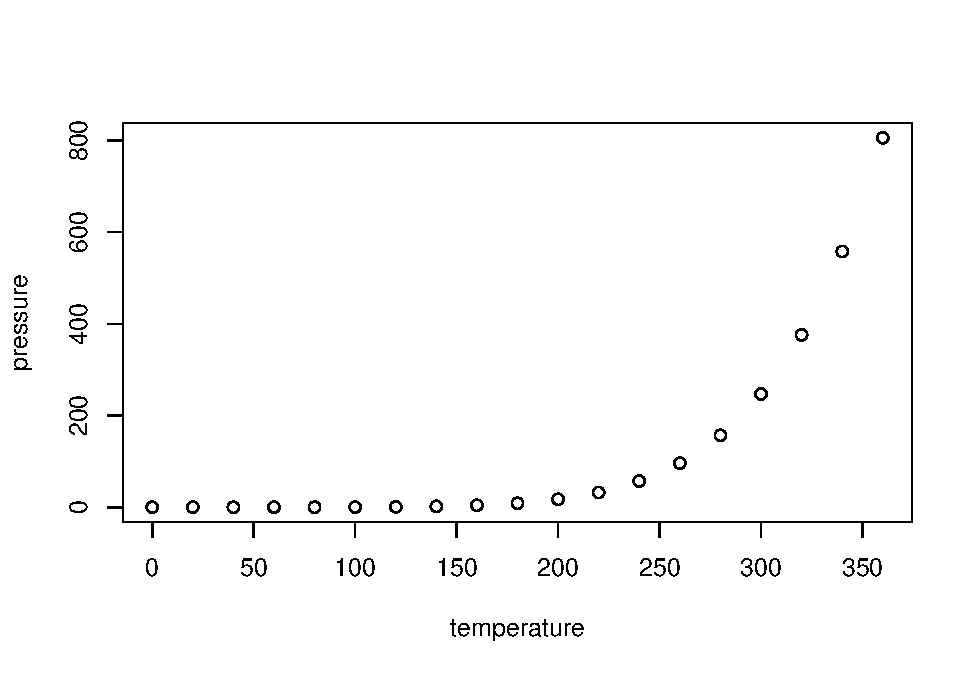
\includegraphics{_main_files/figure-latex/pressure4-1.pdf}

Note that the \texttt{echo\ =\ FALSE} parameter was added to the code chunk to prevent printing of the R code that generated the plot.

\hypertarget{spatiotemporal-tuning}{%
\chapter{Spatiotemporal tuning}\label{spatiotemporal-tuning}}

This is an R Markdown document. Markdown is a simple formatting syntax for authoring HTML, PDF, and MS Word documents. For more details on using R Markdown see \url{http://rmarkdown.rstudio.com}.

When you click the \textbf{Knit} button a document will be generated that includes both content as well as the output of any embedded R code chunks within the document. You can embed an R code chunk like this:

\begin{Shaded}
\begin{Highlighting}[]
\FunctionTok{summary}\NormalTok{(cars)}
\end{Highlighting}
\end{Shaded}

\begin{verbatim}
##      speed           dist       
##  Min.   : 4.0   Min.   :  2.00  
##  1st Qu.:12.0   1st Qu.: 26.00  
##  Median :15.0   Median : 36.00  
##  Mean   :15.4   Mean   : 42.98  
##  3rd Qu.:19.0   3rd Qu.: 56.00  
##  Max.   :25.0   Max.   :120.00
\end{verbatim}

\hypertarget{including-plots-2}{%
\section{Including Plots}\label{including-plots-2}}

You can also embed plots, for example:

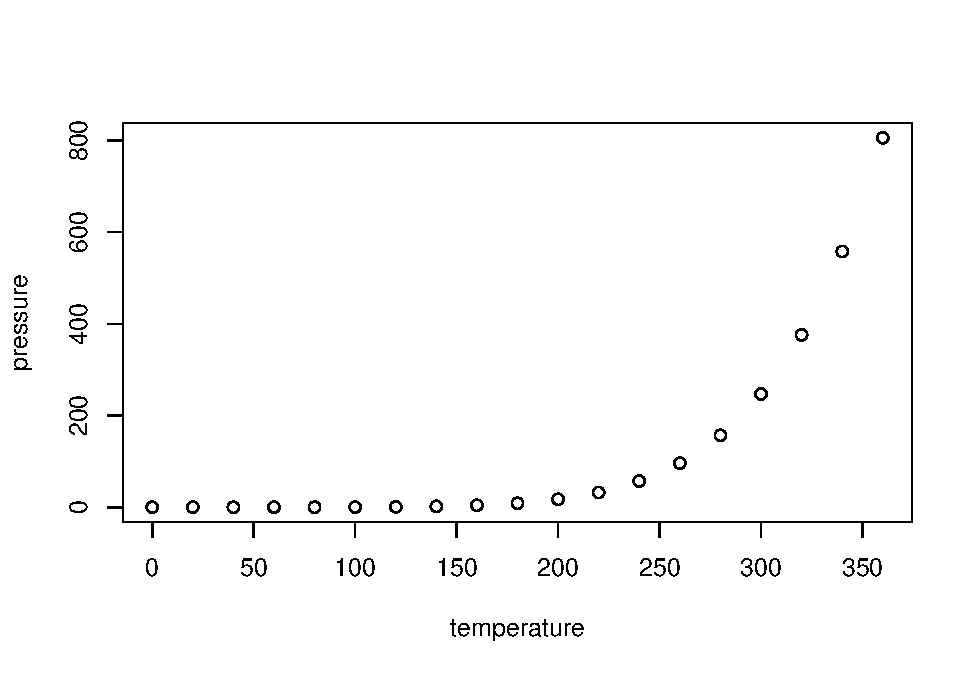
\includegraphics{_main_files/figure-latex/pressure5-1.pdf}

Note that the \texttt{echo\ =\ FALSE} parameter was added to the code chunk to prevent printing of the R code that generated the plot.

\hypertarget{histological-verification}{%
\chapter{Histological verification}\label{histological-verification}}

This is an R Markdown document. Markdown is a simple formatting syntax for authoring HTML, PDF, and MS Word documents. For more details on using R Markdown see \url{http://rmarkdown.rstudio.com}.

When you click the \textbf{Knit} button a document will be generated that includes both content as well as the output of any embedded R code chunks within the document. You can embed an R code chunk like this:

\begin{Shaded}
\begin{Highlighting}[]
\FunctionTok{summary}\NormalTok{(cars)}
\end{Highlighting}
\end{Shaded}

\begin{verbatim}
##      speed           dist       
##  Min.   : 4.0   Min.   :  2.00  
##  1st Qu.:12.0   1st Qu.: 26.00  
##  Median :15.0   Median : 36.00  
##  Mean   :15.4   Mean   : 42.98  
##  3rd Qu.:19.0   3rd Qu.: 56.00  
##  Max.   :25.0   Max.   :120.00
\end{verbatim}

\hypertarget{including-plots-3}{%
\section{Including Plots}\label{including-plots-3}}

You can also embed plots, for example:

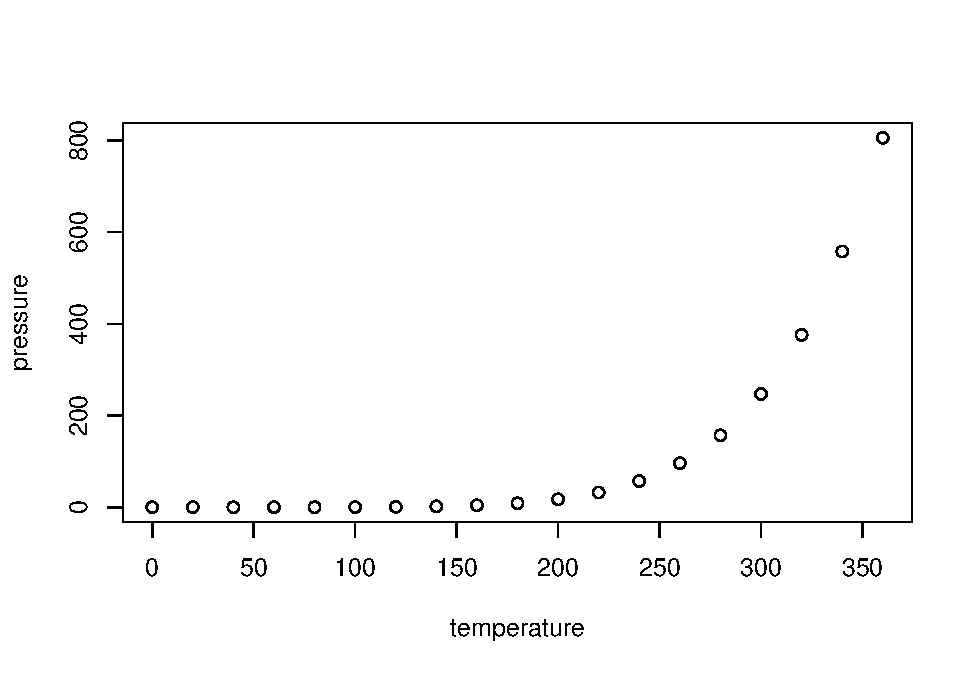
\includegraphics{_main_files/figure-latex/pressure6-1.pdf}

Note that the \texttt{echo\ =\ FALSE} parameter was added to the code chunk to prevent printing of the R code that generated the plot.

  \bibliography{book.bib,packages.bib}

\end{document}
